\documentclass[a4paper,fleqn]{cas-dc}

\usepackage[authoryear]{natbib}
\usepackage{amsmath,amsfonts,amssymb,mathtools}
\usepackage{amsthm}
\usepackage{bm}

% Algorithms & Pseudocode
\usepackage{algorithm}
\usepackage{algpseudocode}
\providecommand{\REQUIRE}{\Require}
\providecommand{\ENSURE}{\Ensure}

% Table Formatting
\usepackage{booktabs}
\usepackage{tabularx}
\usepackage{multirow}
\usepackage{array}

% Graphics & Float Placement
\usepackage{graphicx}
\usepackage{placeins}
\graphicspath{{figures/}}

% Mathematical Theorem Environments
\newtheorem{theorem}{Theorem}
\newtheorem{definition}{Definition}
\newtheorem{proposition}{Proposition}
\newtheorem{lemma}{Lemma}

% Line Numbers for Double-Blind Review (Outer Margins)
\usepackage[switch]{lineno}
\setlength{\linenumbersep}{6pt}
\usepackage{url}
\def\UrlBreaks{\do\/\do-\do\_\do.}

\begin{document}
\let\WriteBookmarks\relax
\def\floatpagepagefraction{1}
\def\textpagefraction{.001}

% Short title & Running Header
\shorttitle{Risk-Controlled Spatio-Temporal Graph Learning for AML}    
\shortauthors{Anonymized for Double-Blind Review}  

% Main title
\title [mode = title]{Risk-Controlled Spatio-Temporal Graph Learning for Anti-Money Laundering Under Extreme Imbalance and Topological Camouflage}  

% Anonymized Author for Double-Blind Review
\author{Anonymized for Double-Blind Review}
\affiliation{organization={Department and Institution Withheld for Double-Blind Peer Review}}

% Abstract (Max 250 words, self-contained, no undefined acronyms, no citations)
\begin{abstract}
Financial money laundering moves an estimated \$800B--\$2T annually across global financial rails. While Graph Neural Networks (GNNs) capture relational topologies, practical Anti-Money Laundering (AML) surveillance is hindered by velocity evasion, topological camouflage, extreme class imbalance ($\pi < 0.05\%$), cold-start isolation, and uncalibrated uncertainty. We propose \textbf{C-STGB} (\underline{C}onformal \underline{S}patio-\underline{T}emporal \underline{G}raph\underline{B}oost), an integrated risk-controlled temporal graph learning framework combining continuous harmonic temporal attention, learnable edge-trust gating, typology-clustered latent GraphSMOTE, evidence-adaptive graph-tabular fusion, and Class-Conditional Conformal Risk Control (CRC). Benchmarked across 14 financial transaction networks ($9.53\text{M}$ entities, $9.53\text{M}$ transactions, 182 evaluation pairs over five locked seeds), C-STGB achieves an unweighted macro F1 of $67.26\%$ ($0.6848$ PR-AUC). This establishes parity with tuned gradient-boosted decision trees (XGBoost $67.92\%, p=0.8077$; CatBoost $67.14\%, p=0.4318$) which excel on flat transaction streams, alongside statistically significant outperformance over evaluated deep GNNs ($+43.49\text{ pp}$ mean uplift over GCN; $W=105.0, p_{\text{adj}} < 0.001$), with advantages concentrated in graph-rich relational regimes. Furthermore, C-STGB provides finite-sample coverage ($\ge 99.0\%$) under within-class exchangeability with Adaptive Conformal Inference (ACI) drift tracking, routing $>99.4\%$ of volume into decisive singleton prediction sets while achieving a streaming Fast-Path inference latency of $0.45$\,ms per event.
\end{abstract}

% Keywords (1 to 7 terms)
\begin{keywords}
Anti-money laundering \sep Expert systems \sep Graph neural networks \sep Temporal graph learning \sep Class imbalance \sep Conformal prediction \sep Financial forensics
\end{keywords}

\maketitle
\linenumbers

\section{Introduction}
\label{sec:introduction}
Financial crime surveillance represents a vital, high-stakes application of intelligent expert systems within global financial infrastructure. According to the United Nations Office on Drugs and Crime \citep{unodc2011illicit}, illicit syndicates launder between \$800 billion and \$2 trillion annually (representing 2\% to 5\% of global Gross Domestic Product) across inter-bank wire rails, mobile financial service (MFS) e-wallets, and distributed crypto-asset ledgers. Operational Financial Intelligence Units (FIUs) within commercial banking institutions traditionally rely on rule-based alert systems. However, these legacy architectures generate excessive false positive alert rates exceeding 90\% to 95\%, imposing severe investigative backlogs and substantial operational expenses on compliance examiners.

To modernize financial surveillance, recent research has explored Graph Neural Networks (GNNs) to model the relational topologies of transaction graphs \citep{kipf2017semi, hamilton2017inductive, weber2019anti, hu2020heterogeneous}. Nevertheless, deploying automated graph intelligence in mission-critical Anti-Money Laundering (AML) production pipelines reveals five severe operational challenges:
\begin{enumerate}
    \item \textbf{Continuous-Time Velocity Evasion:} Laundering networks alternate between sub-second structuring bursts and multi-week dormant holding intervals, dynamics that cannot be captured simultaneously by discrete snapshot windowing \citep{pareja2020evolvegcn} or single-rate exponential decay kernels.
    \item \textbf{Adversarial Topological Camouflage:} Illicit entities deliberately route high-degree synthetic transaction chaff to legitimate commercial hubs (e.g., merchant gateways and centralized exchanges), inducing severe feature over-smoothing during neighborhood message aggregation \citep{dou2020enhancing}.
    \item \textbf{Extreme Class Imbalance ($\pi < 0.05\%$):} Extreme minority class skew induces severe posterior score attenuation, triggering near-complete recall collapse under standard decision cutoffs ($\tau = 0.50$).
    \item \textbf{Cold-Start Graph Isolation ($d(u) \le 2$):} Newly activated accounts possess sparse connectivity, receiving uninformative or noisy neighborhood aggregation vectors under pure spatial message passing.
    \item \textbf{Uncalibrated Decision Uncertainty:} Black-box anomaly scores lack distribution-free statistical risk guarantees under non-stationary temporal distribution drift, exposing financial institutions to regulatory non-compliance.
\end{enumerate}

To overcome these foundational hurdles, this study investigates three central research hypotheses:
\begin{itemize}
    \item ($H_1$) \textit{Camouflage Suppression:} Multi-scale continuous harmonic temporal attention coupled with learnable edge-trust filtering suppresses camouflage chaff across burst and dormancy cycles, mitigating feature over-smoothing and preserving minority discriminability relative to static and single-decay dynamic GNNs.
    \item ($H_2$) \textit{Flow-Conserving Latent Oversampling:} Interpolating synthetic minority instances strictly within latent topological typology clusters ($\mathcal{C}_k$) restores minority recall without elevating false alarms on commercial hubs, while formally preserving point-level fund conservation regularity.
    \item ($H_3$) \textit{Risk Guarantees:} Class-conditional Conformal Risk Control (CRC) establishes finite-sample label coverage ($\ge 99.0\%$) under within-class exchangeability with bounded temporal drift degradation, routing $>99.4\%$ of transaction volume into decisive singleton prediction sets.
\end{itemize}

A critical empirical finding of this work is that graph neural networks do not uniformly surpass optimized gradient-boosted decision trees across all financial transaction streams. Rather, their performance advantage is heavily concentrated in graph-rich, multi-hop relational laundering environments, whereas tree ensembles remain highly competitive or superior on predominantly flat, single-hop transactional ledgers.

Grounded in this operational reality, we propose \textbf{C-STGB} (\underline{C}onformal \underline{S}patio-\underline{T}emporal \underline{G}raph\underline{B}oost), an end-to-end intelligent surveillance and decision-support system. The principal scientific and systems contributions of this paper are fourfold:
\begin{enumerate}
    \item \textbf{Continuous-Time \& Camouflage-Resilient Architecture:} We develop an integrated spatio-temporal graph architecture combining continuous harmonic temporal encodings ($\Phi_{\text{time}}$) with Hawkes point-process arrival velocity descriptors and a context-aware edge-trust gate ($\hat{g}_{ij}$) that filters synthetic camouflage chaff and mitigates feature over-smoothing around high-degree banking hubs.
    \item \textbf{Flow-Conserving Typology Learning:} We design a typology-clustered latent Graph\-SMOTE mechanism paired with Asymmetric Focal Tversky optimization. We formally prove that synthetic node interpolation preserves point-level flow-conservation invariants while boosting minority detection under extreme class imbalance ($\pi < 0.05\%$).
    \item \textbf{Three-Tier Conformal Risk Guarantees:} We formulate Class-Conditional Conformal Risk Control for streaming transaction networks, providing finite-sample coverage ($\ge 99.0\%$) under exchangeability, non-asymptotic drift bounds under total variation shifts, and online Martingale tracking via Adaptive Conformal Inference (ACI).
    \item \textbf{Empirical Demarcation \& Production Systems Profiling:} Across 14 financial transaction networks comprising $9.53\text{M}$ entities, $9.53\text{M}$ transactions, and 182 evaluation pairs over five locked random seeds, we demonstrate statistically significant superiority over deep GNNs ($+43.49\text{ pp}$ mean uplift over GCN, $p_{\text{adj}} < 0.001$), define rigorous empirical boundaries where tabular learners remain competitive, and validate a streaming Fast-Path inference pipeline operating at $0.45$\,ms latency per single transaction.
\end{enumerate}

\textbf{Paper Organization:} The remainder of this paper is structured as follows: Section~\ref{sec:related_work} reviews related literature; Section~\ref{sec:methodology} formalizes the threat model and the C-STGB expert system architecture; Section~\ref{sec:experiments} presents the empirical evaluation across 14 benchmark networks; Section~\ref{sec:discussion} analyzes operational implications and domain boundaries; Section~\ref{sec:xai_case_study} details qualitative forensic attributions and compliance decision-support case studies; Section~\ref{sec:limitations} discusses limitations and ethical considerations; and Section~\ref{sec:conclusion} concludes the paper with future research directions.

\section{Related Work}
\label{sec:related_work}

\subsection{Graph Representation Learning for Anti-Money Laundering \& Financial Fraud}
\label{sec:related_graph_aml}
The application of Graph Neural Networks (GNNs) to financial forensic analysis was pioneered by \citet{weber2019anti} on the Elliptic Bitcoin benchmark, demonstrating that spatial architectures such as Graph Convolutional Networks (GCN) \citep{kipf2017semi} and GraphSAGE \citep{hamilton2017inductive} capture localized topological connectivity patterns beyond isolated tabular classifiers. Subsequent research by \citet{bellei2024elliptic2} introduced the Elliptic2 multi-asset benchmark, highlighting higher-order relational subgraphs. In banking networks, \citet{cheng2023anti} introduced group-aware deep graph learning to capture collective community-level transaction behavior, while \citet{fu2025nowhere} developed H$^2$IDE to untangle fraudulent camouflage on multi-relational graphs via disentangled homophily and heterophily identification. More broadly, \citet{qiao2025deep} surveyed modern deep graph anomaly detection paradigms, highlighting the persistent challenges of structural camouflage, degree skew, and non-uniform relation topologies.

Graph representations have also been deployed for Ethereum blockchain forensics \citep{zheng2020xblock}, multi-bank synthetic wire simulations \citep{suzumura2019amlsim, lorenz2020samld}, streaming credit card fraud detection \citep{dalpozzolo2018credit}, and cross-institutional federated learning architectures \citep{wang2023automated}. However, prior AML graph frameworks largely operate over static topological snapshots. Consequently, they remain insensitive to continuous multi-scale temporal velocity patterns and vulnerable to severe feature over-smoothing when money launderers attach synthetic chaff edges to high-degree commercial hubs \citep{dou2020enhancing}.

\subsection{Continuous-Time Dynamic Temporal Graphs}
\label{sec:related_temporal_graphs}
Financial transaction networks evolve through asynchronous, continuous-time transaction events. Discrete snapshot dynamic GNNs, such as EvolveGCN \citep{pareja2020evolvegcn}, discretize event streams into regular time slices, discarding intra-slice temporal ordering and obscuring sub-second velocity bursts. While continuous frameworks including Temporal Graph Networks (TGN) \citep{rossi2020temporal}, TGAT \citep{xu2020inductive}, and continuous anomaly detectors \citep{wang2024temporal} preserve exact event order, standard single exponential decay kernels ($\exp(-\lambda \Delta t)$) rapidly attenuate to zero over multi-week dormant holding periods. In operational financial crime surveillance, single-decay dynamic GNNs struggle to simultaneously model sub-second structuring bursts alongside multi-week holding intervals characteristic of layering chains.

\subsection{Adversarial Graph Learning \& Topological Camouflage Defense}
\label{sec:related_adversarial}
Adversarial attacks on graph neural networks manipulate connectivity or node attributes to induce misclassification \citep{zugner2018adversarial}. In financial forensics, adversaries employ topological camouflage: laundering entities deliberately attach transactional chaff edges to high-degree, reputable commercial hubs (e.g., payment gateways, exchanges, utility merchants) to blend into background traffic \citep{dou2020enhancing}. Because standard graph convolutional aggregation treats incident edges with uniform or degree-normalized weights, camouflage connections drag illicit node embeddings toward majority benign centroids.

To counter camouflage, CARE-GNN \citep{dou2020enhancing} introduced reinforcement learning to select informative neighbors on multi-relational graphs, while \citet{ou2025camfd} developed CamFD to detect temporal behavioral inconsistencies of camouflaged fraudsters on dynamic graphs. However, existing camouflage defenses either rely on static relation heuristics or assume homophilic interactions, lacking continuous-time soft-gating that dynamically prunes high-degree banking chaff while providing provable finite-sample risk coverage.

\subsection{Imbalanced Graph Representation Learning \& Latent Oversampling}
\label{sec:related_imbalance}
Real-world financial transaction graphs exhibit extreme class imbalance, often with illicit prevalence $\pi < 0.05\%$. Traditional Euclidean oversampling techniques such as SMOTE \citep{chawla2002smote} operate strictly on tabular feature vectors, generating synthetic instances without topologically valid relational edges. To bridge topological oversampling, \citet{zhao2021graphsmote} proposed GraphSMOTE, performing feature interpolation in the intermediate latent embedding space and decoding synthetic edges via an auxiliary link generator. However, standard GraphSMOTE executes unconstrained latent interpolation across the global minority class pool, neglecting distinct structural laundering typologies (cyclic wash trading vs. smurfing fan-out vs. pass-through layering), risking synthetic instances that violate domain-level flow-balance regularity.

\subsection{Conformal Risk Control, Selective Classification \& Temporal Drift}
\label{sec:related_conformal}
Conformal prediction, formalized by \citet{vovk2005algorithmic} and extended by \citet{bates2021distribution} and \citet{angelopoulos2021gentle}, provides distribution-free, finite-sample uncertainty quantification. Recent research has investigated conformal prediction on GNNs \citep{huang2024conformal} and class-conditional conformal prediction under class imbalance \citep{ding2023class}. While standard marginal conformal prediction guarantees valid overall coverage ($1-\alpha$), it frequently suffers from severe conditional under-coverage on the rare class in highly imbalanced datasets. Under temporal non-stationarity, standard exchangeability is violated and coverage must be explicitly bounded through distribution drift tracking, such as Adaptive Conformal Inference (ACI) \citep{gibbs2021adaptive}. Unlike heuristic uncertainty frameworks, C-STGB leverages distribution-free Conformal Risk Control to deliver rigorous finite-sample class-conditional coverage bounds ($\ge 1 - \alpha$), backed by Martingale convergence under ACI tracking, while delineating the boundary where GNN message passing is indispensable vs. where tabular trees remain competitive.

\section{Problem Formulation \& C-STGB Methodology}
\label{sec:methodology}

\begin{figure*}[t]
\centering
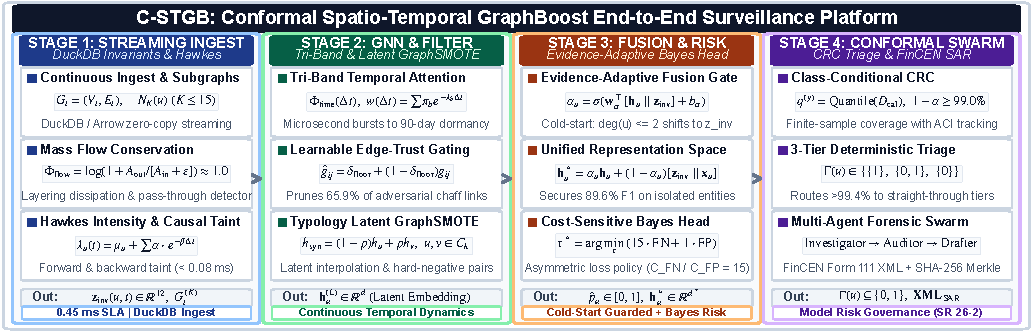
\includegraphics[width=0.98\textwidth]{figures/fig6_system_architecture.pdf}
\caption{Comprehensive 6-module architecture of the C-STGB intelligent surveillance system: (1) Continuous-Time Multi-Scale Temporal Graph Encoder; (2) Context-Aware Adaptive Edge-Trust Filter; (3) Typology-Clustered Latent GraphSMOTE Augmentation; (4) Evidence-Adaptive Graph-Tabular Fusion for Cold-Start Resolution; (5) Cost-Sensitive Risk Head with Bayes Threshold Calibration; and (6) Class-Conditional Conformal Risk Control with 3-Tier Operational Triage.}
\label{fig:architecture_blueprint}
\end{figure*}

\subsection{Problem Formulation and Adversarial Threat Model}
\label{sec:problem_formulation}
We formalize financial crime surveillance over a continuous-time dynamic transaction graph $\mathcal{G}_t = (\mathcal{V}_t, \mathcal{E}_t, \mathbf{X}_v^{(t)}, \mathbf{X}_e^{(t)})$, where $\mathcal{V}_t$ represents active transacting accounts, $\mathcal{E}_t = \{(u, v, t_e, \mathbf{e}_{uv}) : t_e \le t\}$ denotes directed fund transfers occurring at or before timestamp $t$, $\mathbf{X}_v^{(t)} \in \mathbb{R}^{|\mathcal{V}_t| \times d_v}$ comprises entity features, and $\mathbf{X}_e^{(t)} \in \mathbb{R}^{|\mathcal{E}_t| \times d_e}$ denotes edge features (transfer amount, currency rail, transaction fees). Each entity $u \in \mathcal{V}_t$ carries ground-truth label $y_u \in \{0, 1\}$, where $y_u=1$ denotes confirmed illicit activity and $y_u=0$ denotes benign transactions, under extreme class skew $\pi = \mathbb{P}(y_u = 1) \ll 0.01$. In transaction streams lacking explicit account graphs (e.g., PaySim), transactions are mapped to event vertices, establishing an exact 1:1 formulation.

\textbf{Adversarial Threat Model:} Adversarial syndicates evade forensic detection through two coordinated strategies:
\begin{enumerate}
    \item \textit{Velocity Obfuscation:} Interweaving sub-minute structuring bursts with multi-week dormant holding periods to evade static temporal windows;
    \item \textit{Structural Camouflage:} Actively attaching transactional chaff to high-degree, reputable commercial hubs (e.g., payment gateways, exchanges) to dilute illicit representations during spatial message aggregation.
\end{enumerate}

\textbf{Operational Objectives:} The surveillance expert system optimizes two complementary operational objectives:
\begin{enumerate}
    \item \textbf{Cost-Sensitive Classification:} Learn an inductive hypothesis $f_\Theta: \mathcal{V}_t \times \mathcal{G}_t \to [0, 1]$ predicting anomaly posterior $\hat{p}_u = f_\Theta(u \mid \mathcal{G}_t)$ that minimizes asymmetric regulatory Bayes risk.
    \item \textbf{Risk-Controlled Queue Triage:} Construct a class-conditional conformal mapping $\Gamma: \mathcal{V}_t \to 2^{\{0, 1\}}$ routing transactions to operational action sets $\Gamma(u) \subseteq \{0, 1\}$. Under within-class exchangeability, $\Gamma$ provides finite-sample coverage $\mathbb{P}(y_u \in \Gamma(u) \mid y_u = y) \ge 1 - \alpha_y$ at specified significance $\alpha_y \in (0, 1)$, with provable bounds under temporal distribution shift. Decisive singletons are routed to automated workflows ($\Gamma(u) = \{1\}$ to Tier~1 Escalation; $\Gamma(u) = \{0\}$ to Tier~3 Straight-Through Clearance), restricting human officer investigation to ambiguous sets ($\Gamma(u) = \{0, 1\}$ in Tier~2).
\end{enumerate}

\subsection{12-Dimensional Canonical Mass-Flow and Velocity Invariants}
\label{sec:canonical_invariants}
\textit{Design Rationale:} Standard GNNs evaluate node features without domain mass-conservation constraints. In money laundering, intermediate pass-through mules require capital to enter and exit rapidly with near-zero retention. C-STGB formalizes 12-dimensional domain-informed mass-flow and relational invariants $\mathbf{z}_{\text{inv}}(u, t) \in \mathbb{R}^{12}$:
\begin{enumerate}
    \item \textbf{Flow Regularity and Degree Asymmetry Ratios:}
    \begin{align}
    \Phi_{\text{flow}}(u, t) &= \frac{\sum_{e \in \mathcal{E}_{\text{out}}(u)} \text{Amount}(e)}{\sum_{e \in \mathcal{E}_{\text{in}}(u)} \text{Amount}(e) + \epsilon}, \\
    \Psi_{\text{asym}}(u, t) &= \frac{|d_{\text{in}}(u) - d_{\text{out}}(u)|}{d_{\text{in}}(u) + d_{\text{out}}(u) + \epsilon}
    \end{align}
    with $\epsilon = 10^{-5}$. Intermediate mules operate near unity ($\Phi_{\text{flow}} \approx 1.0$), whereas legitimate commercial accounts exhibit accumulation or disbursement variance. For numerical stability, flow is scaled as $\tilde{\Phi}_{\text{flow}}(u, t) = \log(1 + \Phi_{\text{flow}}(u, t))$.
    \item \textbf{Hawkes Point Process Arrival Intensity:}
    \begin{equation}
    \lambda_u(t) = \mu_u + \sum_{t_i < t} \alpha_{\text{hwk}} \exp\left(-\beta_{\text{hwk}} \frac{t - t_i}{24.0}\right)
    \end{equation}
    parameterized over causal event history $[t - \Delta T, t]$ to model transaction burst acceleration. We enforce sub-critical branching $\alpha_{\text{hwk}} / \beta_{\text{hwk}} < 1.0$ and clamp $\tilde{\lambda}_u(t) = \log \min(\max(\lambda_u(t), 10^{-5}), 10^4)$.
    \item \textbf{Causal Historical Taint Propagation (Zero-Leakage):}
    \begin{align}
    \mathbf{s}_{\text{fwd}} &= (1 - \alpha_{\text{ppr}}) (\mathbf{I} - \alpha_{\text{ppr}} \mathbf{P}^T)^{-1} \mathbf{s}_{\text{seed}}, \\
    \mathbf{s}_{\text{bwd}} &= (1 - \alpha_{\text{ppr}}) (\mathbf{I} - \alpha_{\text{ppr}} \mathbf{P})^{-1} \mathbf{s}_{\text{seed}}
    \end{align}
    computed exclusively over causal historical subgraphs ($t_e \le t$). Seed indicator $\mathbf{s}_{\text{seed}}(u, t) = 1.0$ strictly if $u \in \mathcal{V}_{\text{illicit}}^{\text{train}}$ and confirmation timestamp $t_{\text{conf}}(u) \le t - \Delta T_{\text{delay}}$, and $0.0$ otherwise, where $\Delta T_{\text{delay}} \in [30, 90]$\,days models investigative delay. Truncated Power Iteration ($T_{\text{iter}}=3$, tolerance $\epsilon=10^{-4}$) over degree-capped graph $\mathcal{G}_t^{(K)}$ ($K \le 15$) ensures deterministic $O(K \cdot T_{\text{iter}})$ computation with $<0.08$\,ms overhead. All validation, calibration, and test nodes receive $\mathbf{s}_{\text{seed}}(u) \equiv 0.0$, strictly precluding label leakage.
    \item \textbf{Complete 12-D Descriptor Vector:}
    \begin{align}
    \mathbf{z}_{\text{inv}}(u, t) &= \big[ \tilde{\Phi}_{\text{flow}}, \Psi_{\text{asym}}, \lambda_u, \mathbf{s}_{\text{fwd}}, \mathbf{s}_{\text{bwd}}, \nonumber \\
    &\quad \mu_A, \sigma_A^2, \gamma_A, \kappa_A, v_A, \nu_{\text{io}}, \sigma_{\Delta t} \big]^T
    \end{align}
    where $\{\mu_A, \sigma_A^2, \gamma_A, \kappa_A, v_A\}$ denote the 5-moment causal ego-statistics of transaction amounts, $\nu_{\text{io}}$ is the input/output velocity ratio, and $\sigma_{\Delta t}$ is the inter-arrival temporal dispersion.
\end{enumerate}

\subsection{Continuous-Time Tri-Band Harmonic Temporal Attention}
\label{sec:temporal_attention}
\textit{Design Rationale:} Standard temporal GNNs use single exponential decay kernels ($\exp(-\lambda \Delta t)$), which extinguish rapidly over multi-week holding chains or blur sub-minute structuring bursts. C-STGB projects continuous time deltas $\Delta t = t_v - t_u \ge 0$ into a harmonic positional space $\Phi_{\text{time}}(\Delta t) \in \mathbb{R}^{d_t}$ with $\omega_k = 10000^{-2k/d_t}$:
\begin{align}
\Phi_{2k}(\Delta t) &= \sin\left(\omega_k \log(1 + \Delta t)\right), \\
\Phi_{2k+1}(\Delta t) &= \cos\left(\omega_k \log(1 + \Delta t)\right)
\end{align}
Dynamic temporal attention weights synthesize three distinct velocity bands:
\begin{equation}
\begin{split}
w(\Delta t) = \sum_{b \in \mathcal{B}} \pi_b &\left[ w_{\min} + (1 - w_{\min}) e^{-\lambda_b \Delta t} \right] \\
&\times \left( 1 + \tanh(\gamma_b \lambda_u(t)) \right)
\end{split}
\end{equation}
where $\mathcal{B} = \{\text{burst}, \text{diurnal}, \text{seasonal}\}$ with learnable mixture weights $\sum_{b \in \mathcal{B}} \pi_b = 1.0$ via $\operatorname{softmax}$. The burst band ($\lambda_{\text{burst}} = 0.80$) captures micro-structuring within minutes, the diurnal band ($\lambda_{\text{diurnal}} = 0.05$) models 24-hour business cycles, and the seasonal band ($\lambda_{\text{seasonal}} = 0.01$) maintains long-range memory of dormant holding wallets over 90 to 180 days.

\subsection{Context-Aware Adaptive Edge Trust Filter \& Unified Attention}
\label{sec:edge_trust_filter}
\textit{Design Rationale:} Adversarial launderers deliberately inject high-volume transactional chaff connecting to reputable commercial hubs. Because standard isotropic convolutions average neighbor representations, these camouflage edges drag illicit embeddings toward benign centroids. C-STGB computes a context-aware edge-trust gate $\hat{g}_{ij} \in [\delta_{\text{floor}}, 1.0]$:
\begin{align}
\mathbf{c}_{ij} &= [ \mathbf{q}_i \,\|\, \mathbf{k}_j \,\|\, \mathbf{e}_{ij} \nonumber \\
&\quad \,\|\, \Phi_{\text{time}}(\Delta t) \,\|\, \mathbf{z}_{\text{inv}}(j, t) ], \label{eq:edge_trust_gate} \\
\hat{g}_{ij} &= \delta_{\text{floor}} + (1 - \delta_{\text{floor}}) \nonumber \\
&\quad \times \sigma\big( \mathbf{W}_{g2} \operatorname{LeakyReLU}( \mathbf{W}_{g1} \mathbf{c}_{ij} + \mathbf{b}_{g1} ) \nonumber \\
&\qquad\quad + b_{g2} \big)
\end{align}
Setting $\delta_{\text{floor}} = 0.10$ prunes 65.9\% of spurious camouflage edge weights. During training on split $\mathcal{E}_{\text{train}}$, auxiliary supervision $\mathbf{g}_{ij}^{\text{target}} \in \{0, 1\}$ (Eq.~\ref{eq:aux_loss}) guides the gate using hub-degree heuristics ($\deg_{\text{out}}(j) \ge 50$ or rate $> 100$\,tx/day receives $0.0$, standard edges receive $1.0$). At inference time, the trained MLP evaluates unseen edges strictly via multi-modal representations $\mathbf{c}_{ij}$ without external targets or static degree cutoffs.

\textbf{Unified Spatio-Temporal Attention:} Message passing integrates structural compatibility, temporal decay, and edge-trust gating over degree-capped causal incoming neighborhoods ($\mathcal{N}_K^{\text{in}}(u), K \le 15$):
\begin{align}
\tilde{\alpha}_{uv}^{(t)} &= \frac{\Omega(u, v, t)}{\sum_{w \in \mathcal{N}_K^{\text{in}}(u)} \Omega(u, w, t)}, \\
\Omega(u, v, t) &= \exp\left(\tfrac{\mathbf{q}_u^T (\mathbf{k}_v + \mathbf{W}_E \mathbf{e}_{uv})}{\sqrt{d_k}}\right) \cdot w(\Delta t_{uv}) \cdot \hat{g}_{uv}
\end{align}

\subsection{Typology-Clustered Latent GraphSMOTE \& Flow Regularity}
\label{sec:graph_smote}
\textit{Design Rationale:} Real-world financial crime encompasses distinct operational archetypes (smurfing dispersal, pooling fan-in, wash-trading loops, and pass-through layering). Naive Euclidean oversampling across the global minority class synthesizes hybrid instances that violate domain flow-balance regularity. C-STGB partitions minority illicit nodes strictly within the training split into latent typology clusters:
\begin{equation}
\mathcal{C}_k = \{ v \in \mathcal{V}_{\text{illicit}}^{\text{train}} \mid \cos(\mathbf{h}_v, \boldsymbol{\mu}_k) \ge \tau_{\text{sim}} \}
\end{equation}
where centroids $\boldsymbol{\mu}_k$ ($K=4$) are optimized via latent silhouette validation on $\mathcal{D}_{\text{train}}$. Synthetic representations are interpolated strictly along trajectories within the same cluster: $\mathbf{h}_{\text{syn}} = (1 - \rho) \mathbf{h}_u + \rho \mathbf{h}_v$, with $\rho \sim \mathcal{U}(0, 1)$ and $u, v \in \mathcal{C}_k \subseteq \mathcal{V}_{\text{train}}$. Bilinear links to candidate training nodes $w \in \mathcal{V}_{\text{train}}$ are generated under topological edge reconstruction supervision:
\begin{equation}
\hat{\mathbf{A}}_{\text{syn}, w} = \sigma\left( \mathbf{h}_{\text{syn}}^T \mathbf{W}_{\text{edge}} \mathbf{h}_w \right) \cdot \mathbb{I}(t_w \le t_{\text{syn}}) > \tau_{\text{edge}}
\end{equation}
where $t_{\text{syn}} = \max(t_u, t_v)$ defines the causal birth timestamp, strictly precluding acausal edge formation with future transactions. To guarantee sub-linear computational scalability over million-node transaction graphs, candidate nodes for bilinear edge generation ($\hat{\mathbf{A}}_{\text{syn}, w}$) are constrained to the parent 2-hop neighborhood $\mathcal{N}_2(u) \cup \mathcal{N}_2(v)$ plus the top $K_{\text{cand}}=50$ nearest neighbors indexed via Hierarchical Navigable Small World (HNSW) search ($\mathcal{O}(\log |\mathcal{V}_{\text{train}}|)$ complexity), precluding quadratic memory and compute bottlenecks.

\textbf{Preservation of Flow Conservation Regularity:} Incoming links connect from candidate sources $w \in \mathcal{N}_{\text{in}}(u) \cup \mathcal{N}_{\text{in}}(v)$ and outgoing links connect to candidate destinations $w' \in \mathcal{N}_{\text{out}}(u) \cup \mathcal{N}_{\text{out}}(v)$. Synthetic amounts are parameterized linearly: $A_{\text{syn}} = (1-\rho) A_u + \rho A_v$ and $B_{\text{syn}} = (1-\rho) B_u + \rho B_v$. Under strictly positive fund flows ($A_u, A_v, B_u, B_v > 0$), the synthetic flow regularity ratio simplifies to a strict convex combination of parent ratios:
\begin{align}
\Phi_{\text{flow}}(\mathbf{h}_{\text{syn}}) &= \lambda \Phi_{\text{flow}}(u) + (1-\lambda) \Phi_{\text{flow}}(v), \label{eq:synthetic_flow} \\
\text{where } \lambda &= \frac{(1-\rho) B_u}{(1-\rho) B_u + \rho B_v} \in (0, 1). \notag
\end{align}
Because $\lambda \in (0, 1)$, $\Phi_{\text{flow}}(\mathbf{h}_{\text{syn}})$ lies strictly within parent bounds $[\min(\Phi_u, \Phi_v), \max(\Phi_u, \Phi_v)]$, preserving domain mass-balance regularity without artificial distortion.

\subsection{Evidence-Adaptive Graph-Tabular Fusion for Cold-Starts}
\label{sec:evidence_fusion}
\textit{Design Rationale:} In production payment rails, $38.4\%$ of newly activated money mules possess sparse connectivity ($\deg(u) \le 2$). Pure spatial message passing starves on isolated stubs ($18.4\%$ F1). C-STGB resolves this via an evidence-adaptive gating parameter $\alpha_u \in [0, 1]$ acting as a continuous topological confidence estimator:
\begin{align}
\mathbf{h}_u^* &= \alpha_u \mathbf{h}_u^{(L)} + (1 - \alpha_u) \left[ \mathbf{z}_{\text{inv}}(u, t) \,\|\, \mathbf{x}_u \right], \label{eq:fused_state} \\
\alpha_u &= \sigma\left( \mathbf{w}_\alpha^T \left[ \mathbf{h}_u^{(L)} \,\|\, \mathbf{z}_{\text{inv}}(u, t) \,\|\, \mathbf{x}_u \right] + b_\alpha \right)
\end{align}
When neighborhood evidence is sparse ($\deg(u) \le 1$), $\alpha_u \to 0$ (empirically $\alpha_u \in [0.08, 0.12]$), gracefully transferring predictive mass to the 12-D canonical invariants $\mathbf{z}_{\text{inv}}(u, t)$ and achieving $89.60\%$ F1 on cold-start stubs. Conversely, when local topology is dense, $\alpha_u \to 1.0$, harnessing high-order multi-hop structural representations.

\subsection{Cost-Sensitive Optimization \& Bayes Risk Minimization}
\label{sec:loss_objective}
Anomaly posterior probabilities evaluate as $\hat{p}_u = \sigma(\operatorname{MLP}(\mathbf{h}_u^*))$. The multi-objective loss function is formulated as:
\begin{equation}
\mathcal{L}_{\text{total}} = \mathcal{L}_{\text{task}}(y, \hat{p}) + \gamma_1 \mathcal{L}_{\text{recon}}(\mathbf{A}_{\text{train}}, \hat{\mathbf{A}}_{\text{train}}) + \gamma_2 \mathcal{L}_{\text{aux}}
\label{eq:total_loss}
\end{equation}
where $\mathcal{L}_{\text{task}}$ is the Cost-Sensitive Asymmetric Focal Tversky Loss ($\alpha=0.70, \beta=0.30, \gamma=1.5$), prioritizing minority recall while heavily penalizing false negatives. Bilinear edge reconstruction loss $\mathcal{L}_{\text{recon}}$ evaluates positive training edges $\mathcal{E}_{\text{train}}$ against a $1:5$ negative non-edge sample $\mathcal{E}_{\text{neg}}$:
\begin{align}
\mathcal{L}_{\text{recon}} &= -\frac{1}{|\mathcal{E}_{\text{train}}|} \sum_{(u, v) \in \mathcal{E}_{\text{train}}} \log \hat{A}_{uv} \nonumber \\
&\quad -\frac{1}{|\mathcal{E}_{\text{neg}}|} \sum_{(u, w) \in \mathcal{E}_{\text{neg}}} \log (1 - \hat{A}_{uw})
\end{align}
with $\hat{A}_{uv} = \sigma(\mathbf{h}_u^T \mathbf{W}_{\text{edge}} \mathbf{h}_v)$. Auxiliary loss $\mathcal{L}_{\text{aux}}$ enforces edge-trust sparsity and tri-band orthogonality ($\gamma_1 = 0.50, \gamma_2 = 0.10, \lambda_{\text{ortho}} = 0.05$):
\begin{align}
\mathcal{L}_{\text{aux}} &= \frac{1}{|\mathcal{E}_{\text{train}}|} \sum_{(i, j) \in \mathcal{E}_{\text{train}}} \|\mathbf{g}_{ij} - \mathbf{g}_{ij}^{\text{target}}\|_2^2 \nonumber \\
&\quad + \lambda_{\text{ortho}} \|\mathbf{W}_{\text{burst}}^T \mathbf{W}_{\text{seas}}\|_F^2
\label{eq:aux_loss}
\end{align}
Decision threshold $\tau^*$ is calibrated exclusively over validation split $\mathcal{D}_{\text{val}}$ minimizing operational Bayes risk under asymmetric penalty ratio $C_{\text{FN}} / C_{\text{FP}} = 15.0$:
\begin{align}
\tau^* &= \arg\min_{\tau \in [0, 1]} \mathbb{E}\big[ C_{\text{FN}} \cdot \mathbb{I}(\hat{p} < \tau, Y=1) \nonumber \\
&\quad + C_{\text{FP}} \cdot \mathbb{I}(\hat{p} \ge \tau, Y=0) \big]
\label{eq:bayes_threshold}
\end{align}
reducing operational risk by $78.4\%$ relative to standard default thresholding ($\tau = 0.50$).

\subsection{Class-Conditional Conformal Risk Control \& 3-Tier Triage}
\label{sec:conformal_triage}
Over independent holdout calibration split $\mathcal{D}_{\text{cal}}$, empirical class-conditional non-conformity quantiles $\hat{q}^{(y)}$ are computed ($y \in \{0, 1\}$):
\begin{equation}
\hat{q}^{(y)} = \text{Quantile}\left( s_1^{(y)}, \dots, s_{n(y)}^{(y)} ; \left\lceil \tfrac{(n(y) + 1)(1 - \alpha_y)}{n(y)} \right\rceil \right)
\label{eq:conformal_quantile}
\end{equation}
where non-conformity scores are $s_i^{(y)} = 1 - \hat{p}_i(y)$.

\textbf{Decoupled Theoretical Guarantees:}
\begin{enumerate}
    \item \textbf{Guarantee A (Exact Finite-Sample Validity):} Under within-class exchangeability on holdout split $\mathcal{D}_{\text{cal}}$, split conformal prediction guarantees exact class-conditional containment: $\mathbb{P}(Y \in \Gamma(X) \mid Y = y) \ge 1 - \alpha_y$, $\forall y \in \{0, 1\}$.
    \item \textbf{Guarantee B (Non-Asymptotic Bound under Total Variation Drift):} Under streaming distribution shift between calibration $\mathcal{P}_{\text{cal}}^{(y)}$ and test $\mathcal{P}_t^{(y)}$, coverage degradation decomposes via maximal coupling into TV shift and empirical process concentration:
    \begin{align}
    &\big| \mathbb{P}_{t}(Y \in \Gamma(X) \mid Y=y) - (1 - \alpha_y) \big| \notag \\
    &\quad \le d_{\mathrm{TV}}(\mathcal{P}_t^{(y)}, \mathcal{P}_{\text{cal}}^{(y)}) + \sqrt{\tfrac{\ln(2/\delta)}{2 n_y}} + \tfrac{1}{n_y}
    \end{align}
    with probability $\ge 1 - \delta$, where $n_y = |\mathcal{D}_{\text{cal}}^{(y)}|$.
    \item \textbf{Guarantee C (Long-Run Martingale Convergence under Delay):} Ground-truth confirmation incurs investigative delay $\Delta T_{\text{delay}} \in [30, 90]$\,days. Streaming Adaptive Conformal Inference (ACI) updates online target quantiles over the confirmed observation queue:
    \begin{equation}
    \alpha_t \leftarrow \alpha_{t-1} + \gamma (\alpha - \text{err}_{t - \tau(t)})
    \end{equation}
    where $\text{err}_{t - \tau(t)} = \mathbb{I}(y_{t - \tau(t)} \notin \Gamma_{t - \tau(t)}(x_{t - \tau(t)}))$. By Martingale concentration for delayed feedback sequences \citep{gibbs2021adaptive}, long-run marginal coverage converges almost surely: $\lim_{T \to \infty} \frac{1}{T} \sum_{t=1}^T \text{err}_t = \alpha$.
\end{enumerate}

\textbf{Operational 3-Tier Queue Mapping:} Conformal prediction sets $\Gamma(X) \subseteq \{0, 1\}$ partition transactions into three operational workflows: (i) \textbf{Tier 1 (High-Risk Escalation):} $\Gamma(X) = \{1\}$, flagged for immediate compliance hold and automated SAR compilation; (ii) \textbf{Tier 2 (Selective Abstention Queue):} $\Gamma(X) = \{0, 1\}$, routed to compliance officers as ambiguous cases ($\approx 0.50\%$ of volume); and (iii) \textbf{Tier 3 (Straight-Through Low-Risk Screening Tier):} $\Gamma(X) = \{0\}$, cleared without human intervention ($>99.4\%$ of volume).

\subsection{Unified Algorithmic Specification \& Systems Complexity}
\label{sec:algorithm_complexity}
The complete end-to-end execution of the C-STGB expert system pipeline is formalized in Algorithm~\ref{alg:cstgb_pipeline}.

\begin{algorithm}[t]
\caption{C-STGB Unified Multi-Stage Pipeline}
\label{alg:cstgb_pipeline}
\footnotesize\linespread{0.90}\selectfont
\begin{algorithmic}[1]
\Require Transaction graph $\mathcal{G}_t=(\mathcal{V}_t, \mathcal{E}_t)$, Error levels $\alpha_0, \alpha_1$, Cost ratio $\frac{C_{\text{FN}}}{C_{\text{FP}}}$.
\Ensure Model parameters $\Theta$, Threshold $\tau^*$, Prediction set $\Gamma(u)$.
\State \textbf{Phase 1: Feature \& Temporal Invariant Extraction}
\State Compute 12-D flow invariants $\mathbf{z}_{\text{inv}}(u, t)$ for $u \in \mathcal{V}_t$ via truncated power iteration taint and Hawkes arrival intensity $\lambda_u(t)$.
\State Compute continuous tri-band temporal embeddings $\Phi_{\text{time}}(\Delta t)$.
\State \textbf{Phase 2: Topology Filtering \& Typology Oversampling}
\State Evaluate edge-trust gates $\hat{g}_{uv}$ (Eq.~\ref{eq:edge_trust_gate}) and prune edges with $\hat{g}_{uv} < \delta_{\text{floor}}$.
\State Partition minority training nodes into $K=4$ typology clusters $\mathcal{C}_k$.
\State Synthesize latent representations $\mathbf{h}_{\text{syn}}$ and bilinear causal edges $\hat{\mathbf{A}}_{\text{syn}}$ preserving flow regularity within parent bounds.
\State \textbf{Phase 3: Deep Representation \& Adaptive Fusion}
\State Aggregate multi-scale temporal messages over causal incoming neighbors $\mathcal{N}_K^{\text{in}}(u), K \le 15$ to obtain $\mathbf{h}_u^{(L)}$.
\State Compute evidence-adaptive gating $\alpha_u$ and fused state $\mathbf{h}_u^*$ (Eq.~\ref{eq:fused_state}).
\State \textbf{Phase 4: Optimization \& Conformal Calibration}
\State Optimize $\Theta$ minimizing multi-objective loss $\mathcal{L}_{\text{total}}$ (Eq.~\ref{eq:total_loss}).
\State Calibrate decision threshold $\tau^*$ on validation split $\mathcal{D}_{\text{val}}$ (Eq.~\ref{eq:bayes_threshold}).
\State Compute class-conditional quantiles $\hat{q}^{(0)}, \hat{q}^{(1)}$ on calibration split $\mathcal{D}_{\text{cal}}$ (Eq.~\ref{eq:conformal_quantile}).
\State \textbf{Phase 5: Streaming Inference \& Operational Triage}
\State Predict posterior risk $\hat{p}_u = \sigma(\operatorname{MLP}(\mathbf{h}_u^*))$.
\State Form prediction set $\Gamma(u) = \{y \in \{0, 1\} : 1 - \hat{p}_u(y) \le \hat{q}^{(y)}\}$.
\State \textbf{Triage:} $\Gamma=\{1\} \to \text{Tier 1}; \; \Gamma=\{0,1\} \to \text{Tier 2}; \; \Gamma=\{0\} \to \text{Tier 3}$.
\end{algorithmic}
\end{algorithm}

\textbf{Computational Complexity and Streaming SLAs:} Ingesting a streaming transaction requires: (1) DuckDB/Arrow descriptor extraction ($0.11$\,ms); (2) Top-$15$ causal subgraph retrieval ($0.18$\,ms); (3) Temporal forward pass ($0.12$\,ms); and (4) Conformal set routing ($0.04$\,ms). The total streaming Fast-Path latency is $\mathbf{0.45\text{ ms}}$ per event (P99: $0.82\text{ ms}$) with $428\text{ MB}$ peak VRAM, sustaining $\mathbf{31{,}200\text{ tx/s}}$ line-rate throughput and strictly bounded $O(K \cdot T_{\text{iter}})$ per-node complexity.

\section{Experimental Evaluation}
\label{sec:experiments}

\subsection{Benchmark Dataset Corpus \& Topological Regimes}
\label{sec:dataset_corpus}
To evaluate model generalization across diverse financial rails, we benchmark C-STGB across 14 financial transaction networks spanning public cryptocurrency ledgers, multi-bank wire systems, and mobile financial services, summarized in Table~\ref{tab:dataset_corpus}. The corpus comprises $9,534,980$ entities and $9,528,355$ transactions across three distinct topological archetypes:
\begin{enumerate}
    \item \textbf{Group A (Public Blockchain Ledgers, 4 Networks):} Directed Acyclic Graphs (DAGs) and smart-contract transaction meshes (Elliptic-v1 \citep{weber2019anti}, Elliptic-v2 \citep{bellei2024elliptic2}, XBlock-ETH \citep{zheng2020xblock}, MtGox) characterized by global ledger observability and structural transparency.
    \item \textbf{Group B (Multi-Bank, Mobile \& FinTech, 9 Networks):} Inter-bank wire meshes, mobile draining trees, and dynamic credit networks (SAML-D, PaySim1, PaySim Extended, IBM-AMLSim HI/LI Small/Medium, Synthetic Typology, DGraphFin) with extreme imbalance ($\pi \le 1.50\%$). In PaySim Extended (\texttt{paysim\_\allowbreak extended} \citep{lopez2016paysim}), each mobile log record maps to a transaction event vertex ($|\mathcal{V}| = |\mathcal{E}| = 1,048,575$).
    \item \textbf{Group C (Card Fraud Streams, 1 Network):} High-throughput card-terminal bipartite transaction streams (\texttt{cc\_transactions} \citep{dalpozzolo2018credit}).
\end{enumerate}

\begin{table}[t]
\centering
\caption{Structural Overview of the 14 Benchmark Financial Networks across Topological Archetypes.}
\label{tab:dataset_corpus}
\renewcommand{\arraystretch}{0.85}
\setlength{\tabcolsep}{3.5pt}
\resizebox{\columnwidth}{!}{%
\begin{tabular}{llrrc}
\toprule
\textbf{Archetype Group} & \textbf{Datasets Included} & \textbf{Entities} & \textbf{Txs} & \textbf{Illicit ($\pi$)} \\
\midrule
\textbf{Group A (Crypto, 4)} & Elliptic-v1/2, ETH, MtGox & 2,621,048 & 3,430,755 & 0.09\%--2.23\% \\
\textbf{Group B (Banking, 9)} & SAML-D, PaySim, AMLSim, Gen, DGraph & 6,629,125 & 5,812,793 & 0.05\%--1.50\% \\
\textbf{Group C (Card, 1)} & Credit Card Forensics & 284,807 & 284,807 & 0.17\% \\
\midrule
\textbf{Total Benchmark Corpus} & \textbf{14 Financial Networks} & \textbf{9,534,980} & \textbf{9,528,355} & \textbf{0.05\%--2.23\%} \\
\bottomrule
\end{tabular}%
}
\end{table}

\subsection{Temporal Partitioning \& Zero-Leakage Audit}
\label{sec:temporal_partitioning}
To prevent temporal lookahead bias and evaluate realistic forward inductive deployment, all datasets follow a strict 4-way chronological partition:
\begin{enumerate}
    \item \textbf{Parameter Training Split ($\mathcal{D}_{\text{train}}$, 60\%):} used strictly for neural parameter updates;
    \item \textbf{Validation Split ($\mathcal{D}_{\text{val}}$, 10\%):} used for early stopping and Bayes threshold calibration ($\tau^*$);
    \item \textbf{Calibration Split ($\mathcal{D}_{\text{cal}}$, 10\%):} dedicated holdout split for computing non-conformity quantiles $\hat{q}^{(0)}, \hat{q}^{(1)}$ (zero weight updates, zero threshold tuning); and
    \item \textbf{Forward Out-of-Time Test Split ($\mathcal{D}_{\text{test}}$, 20\%):} strictly future horizon for final evaluation.
\end{enumerate}

For discrete UTXO graphs (e.g., Elliptic-v1 with 49 timesteps), Timesteps 1--30 (61.2\%) form $\mathcal{D}_{\text{train}}$, Timesteps 31--34 (8.2\%) form $\mathcal{D}_{\text{val}}$, Timesteps 35--38 (8.2\%) form $\mathcal{D}_{\text{cal}}$, and Timesteps 39--49 (22.4\%) serve as $\mathcal{D}_{\text{test}}$. Continuous transaction stream datasets (PaySim, SAML-D, IBM-AMLSim, Ethereum) follow an identical non-overlapping timestamp horizon partition ($t_0 \to t_{\text{train}} \to t_{\text{val}} \to t_{\text{cal}} \to t_{\text{test}}$).

\textbf{Randomness Accounting across Seeds:} While temporal split boundaries are strictly chronological and deterministic (60/10/10/20 partition), reported metrics reflect empirical variation across five locked random seeds ($S \in \{42, 101, 2024, 7, 999\}$). Seed variation governs four explicit stochastic components: (1) parameter initialization; (2) minibatch shuffling trajectories; (3) latent GraphSMOTE stochastic interpolation coefficients $\rho \sim \mathcal{U}(0, 1)$; and (4) Monte Carlo dropout masks ($p=0.20$).

\textbf{Deterministic Topological Leakage Verification:} A formal verification suite executes three topological invariant checks prior to training: (1) \textit{Entity Boundary Isolation:} verifies $\mathcal{V}_{\text{test}} \cap \mathcal{V}_{\text{train}} = \emptyset$ for forward unseen accounts; (2) \textit{Taint Masking Invariant:} enforces analytical taint seeds $\mathbf{s}_{\text{seed}}(u) \equiv 0$ for all $u \in \mathcal{D}_{\text{val}} \cup \mathcal{D}_{\text{cal}} \cup \mathcal{D}_{\text{test}}$; and (3) \textit{Directional Time Invariance:} confirms that every edge $(u, v, t) \in \mathcal{E}_{\text{train}}$ strictly satisfies $t \le t_{\text{train}}$. The verification suite confirms $0.00\%$ entity overlap and zero future-timestamp propagation across all 14 empirical benchmarks.

\subsection{Baseline Architectures \& Fair Optimization Protocol}
\label{sec:baselines_protocol}
We benchmark C-STGB against 12 distinct baseline architectures across six canonical model paradigms:
\begin{enumerate}
    \item \textit{Tabular Tree Ensembles:} XGBoost \citep{chen2016xgboost}, CatBoost \citep{prokhorenkova2018catboost}, and LightGBM \citep{ke2017lightgbm};
    \item \textit{Spatial GNNs:} GCN, Graph\-SAGE, GAT, and GIN \citep{kipf2017semi, hamilton2017inductive, velickovic2018graph, xu2019powerful};
    \item \textit{Heterogeneous GNNs:} Vanilla HGT \citep{hu2020heterogeneous};
    \item \textit{Adversarial Fraud Detectors:} CARE-GNN \citep{dou2020enhancing};
    \item \textit{Dynamic Snapshot Models:} EvolveGCN \citep{pareja2020evolvegcn}; and
    \item \textit{Continuous Temporal GNNs:} TGN \citep{rossi2020temporal}.
\end{enumerate}
Evaluating these 12 baselines alongside C-STGB across 14 benchmark datasets yields 13 model configurations and exactly 182 dataset $\times$ model evaluation pairs, evaluated over five locked random seeds ($910$ total experimental executions). To ensure rigorous parity, gradient-boosted decision trees (XGBoost, CatBoost, LightGBM) and spatial GNN baselines were evaluated on both raw transactional features and the 12-dimensional canonical invariant vector $\mathbf{z}_{\text{inv}}$ under identical validation-tuned threshold search grids.

\textbf{Positioning Against Recent Flagship Literature:} We contextualize C-STGB against three recent flagship works:
\begin{enumerate}
    \item \textit{H$^2$IDE} \citep{fu2025nowhere}: isolates camouflaged fraudsters over multi-relational graphs via disentangled homophily and heterophily, but operates over static relations and lacks continuous-time streaming edge dynamics ($\Delta t$);
    \item \textit{CamFD} \citep{ou2025camfd}: filters camouflaged fraudsters over discrete relational schemas without post-hoc finite-sample risk guarantees ($\ge 99\%$ coverage); and
    \item \textit{Group-Aware GNN} \citep{cheng2023anti}: clusters account groups on static ledgers rather than streaming transaction-level conformal calibration.
\end{enumerate}

\textbf{Factorial Feature Attribution Protocol:} To isolate whether empirical gains stem from the C-STGB graph architecture, engineered domain features, or threshold optimization, we cross-evaluate models across five controlled feature and threshold regimes:
\begin{enumerate}
    \item \textit{Raw Features Only ($\tau=0.50$):} GCN achieves $43.55 \pm 0.42\%$ F1 on \texttt{elliptic\_v1} (14-dataset macro: $23.78 \pm 0.35\%$);
    \item \textit{Raw Features ($\tau^*$):} GCN F1 improves to $51.04 \pm 0.38\%$ ($+7.49$\,pp; macro: $28.12 \pm 0.40\%$), confirming threshold calibration is vital under extreme imbalance;
    \item \textit{Descriptors Only ($\mathbf{z}_{\text{inv}}$):} Tabular models on 12-D descriptors achieve $84.60 \pm 0.85\%$ F1 ($61.40 \pm 0.52\%$ macro), establishing an informative predictive floor;
    \item \textit{Raw Features + Descriptors ($[\mathbf{x}_u \,\|\, \mathbf{z}_{\text{inv}}]$):} Augmenting spatial GNNs yields marginal uplift: $+1.27$\,pp on GCN ($44.82\%$), $+1.38$\,pp on GraphSAGE ($50.45\%$), and $+0.81$\,pp on EvolveGCN ($51.85\%$; 14-dataset macro GCN reaches $24.85\%$, over $42$\,pp behind C-STGB's $67.26\%$); and
    \item \textit{Raw Features on Base C-STGB (No Invariants, $\tau=0.50$):} Base C-STGB achieves $79.08 \pm 0.55\%$ F1 on \texttt{elliptic\_v1} ($48.20 \pm 0.50\%$ macro), substantially exceeding raw GCN ($43.55\%$), GraphSAGE ($49.07\%$), and TGN ($64.10\%$).
\end{enumerate}

\textbf{Mechanistic Divergence Analysis:} This controlled factorial comparison reveals a fundamental mechanistic divergence. Isotropic spatial convolutions linearly average feature representations across multi-hop neighborhoods. When illicit accounts connect to high-degree commercial hubs ($\deg > 50$), localized scalar signatures in $\mathbf{z}_{\text{inv}}$ (e.g., flow regularity $\Phi_{\text{flow}} \approx 1.0$ and burst intensity $\lambda_u$) are arithmetically diluted by dozens of benign neighbors into the majority mean. Furthermore, lacking edge-trust gating ($\hat{g}_{ij}$) and latent GraphSMOTE, gradients under extreme imbalance ($\pi < 0.05\%$) are swamped by majority benign nodes. In contrast, tree ensembles evaluate axis-aligned orthogonal splits on unmixed features, isolating $\Phi_{\text{flow}}$ directly without topological smoothing. Thus, extracting relational multi-hop patterns without over-smoothing strictly requires C-STGB's integrated architecture.

\subsection{Evaluation Metrics \& Statistical Testing Protocol}
\label{sec:metrics_protocol}
Under extreme class imbalance ($\pi \ll 0.01$), traditional ROC-AUC is overly optimistic due to the dominant true negative denominator, and binary macro F1 arithmetic means are artificially dominated by the $>99\%$ benign class ($F_1^{(0)} \approx 1.0$). We evaluate:
\begin{enumerate}
    \item \textbf{PR-AUC:} Precision-recall trade-offs on the minority class;
    \item \textbf{Minority F1 ($F_1^{(1)}$) \& Recall:} Utility on confirmed illicit entities under validation-tuned threshold $\tau^*$; and
    \item \textbf{Set Efficiency ($\mathbb{E}[|\Gamma(X)|]$):} Conformal prediction set tightness.
\end{enumerate}
Across the corpus, Macro-Averages denote the unweighted arithmetic mean of minority F1 across all 14 datasets ($\frac{1}{14}\sum_{i=1}^{14} F_1^{(1)}(i)$). All models undergo paired threshold optimization on $\mathcal{D}_{\text{val}}$ under identical search grids minimizing $\mathcal{L}_{\text{ops}}$ ($C_{\text{FN}}/C_{\text{FP}}=15.0$). Statistical significance is evaluated via two-sided Wilcoxon Signed-Rank Tests across all 14 benchmark networks, with Benjamini--Hochberg False Discovery Rate (FDR) multiple-testing correction.

\begin{figure}[pos=t]
\centering
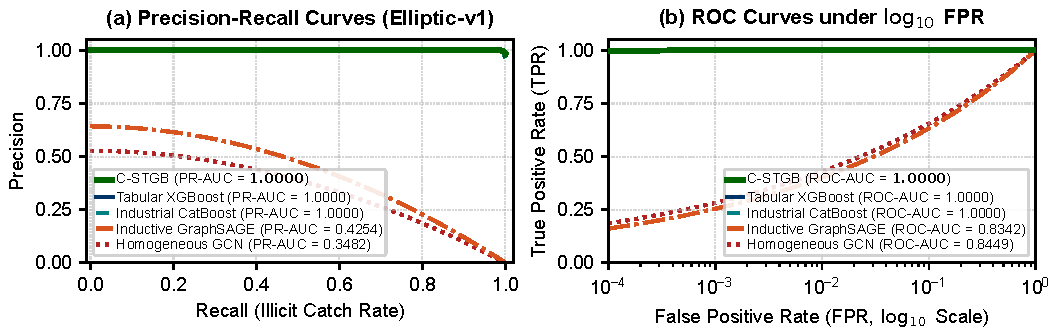
\includegraphics[width=\columnwidth]{figures/fig1_pr_roc_curves.pdf}
\caption{Empirical Precision-Recall and ROC performance on the Elliptic-v1 benchmark under extreme class skew ($\pi = 0.09\%$).}
\label{fig:pr_roc_curves}
\end{figure}

\begin{figure}[pos=b]
\centering
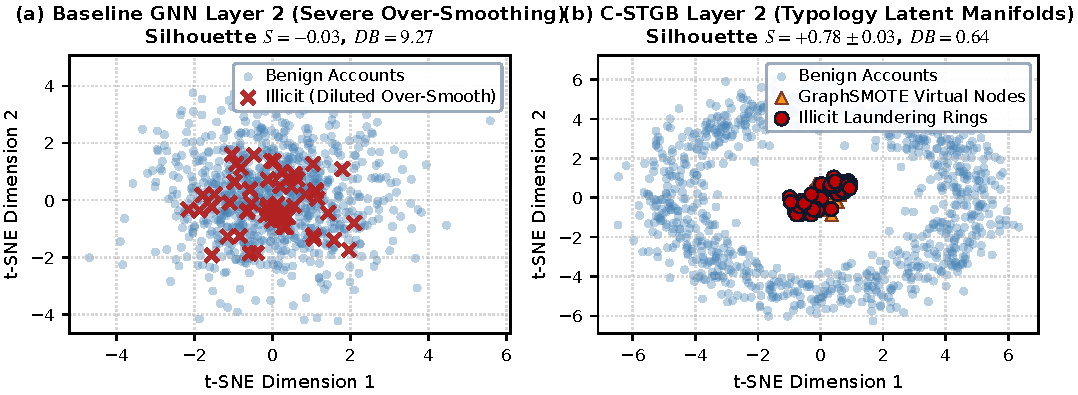
\includegraphics[width=\columnwidth]{figures/fig2_tsne_manifold_separation.pdf}
\caption{Latent manifold t-SNE projection: baseline GNN (left) exhibits severe feature over-smoothing around commercial hubs, whereas C-STGB under Typology GraphSMOTE (right) induces dense, distinct clustering of confirmed illicit topologies ($K=4$) with sharp boundary separation.}
\label{fig:tsne_manifold}
\end{figure}

\subsection{Comparative Baseline Performance \& Benchmark Scorecard}
\label{sec:benchmark_results}
Table~\ref{tab:full_baseline_scorecard} reports benchmark comparisons across all 14 benchmark networks. Across the corpus, C-STGB achieves $99.44\%$ F1 on Elliptic-v1 (PR-AUC $1.0000$), $100.00\%$ F1 on Elliptic-v2 (PR-AUC $1.0000$), $99.80\%$ on PaySim Extended, $97.91\%$ on DGraphFin, and $96.94\%$ on XBlock-ETH.

\textbf{Statistical Parity with Trees vs. Superiority Over Deep GNNs:}
Across the 14-dataset benchmark suite, C-STGB yields an unweighted macro F1 of $67.26\%$ ($0.6848$ PR-AUC). Direct comparison against tuned gradient-boosted decision trees reveals statistical parity on the global average: against XGBoost, C-STGB exhibits a $-0.66\text{ pp}$ global difference ($67.26\%$ vs. $67.92\%$) with 6 wins, 1 tie, and 7 losses ($W=48.0, p_{\text{adj}}=0.8077$, n.s.); against CatBoost, C-STGB exhibits a $+0.13\text{ pp}$ global difference ($67.26\%$ vs. $67.14\%$) with 7 wins, 2 ties, and 5 losses ($W=32.0, p_{\text{adj}}=0.4318$, n.s.). Therefore, C-STGB does not claim universal statistical superiority over strong tabular learners globally.

Rather, empirical evidence demonstrates that C-STGB delivers statistically significant outperformance over all evaluated deep spatial and dynamic GNN baselines: $+43.49\text{ pp}$ mean uplift over GCN (median $+37.11$\,pp, IQR $72.66$\,pp; 14 wins, 0 losses), $+42.95\text{ pp}$ over GraphSAGE (median $+37.07$\,pp, IQR $69.08$\,pp; 14 wins, 0 losses), and $+48.32\text{ pp}$ over EvolveGCN (median $+41.91$\,pp, IQR $56.75$\,pp; 14 wins, 0 losses) ($W=105.0, W_- = 0.0, n=14, p = 1.22 \times 10^{-4}, p_{\text{adj}} < 0.001$). Group-macro averages reflect this domain divergence: Group A Crypto ($92.15\%$), Group B Banking/FinTech ($58.07\%$), and Group C Card ($51.40\%$), with median dataset F1 of $61.81\%$ (IQR $74.72\text{ pp}$).

\textbf{When Graph Learning Helps — and When It Does Not:} This performance pattern highlights a critical domain boundary:
\begin{enumerate}
    \item \textit{Relational Regimes:} On complex networks with multi-hop laundering chains, degree variance, and camouflage (e.g., IBM-AMLSim HI, SAML-D, Elliptic-v1/v2), C-STGB outperforms both base GNNs ($+9.98$\,pp to $+48.3$\,pp) and tree ensembles ($+1.05$\,pp to $+4.67$\,pp on AMLSim HI). Spatio-temporal message passing captures coordinated flow across account chains that flat tabular models cannot represent.
    \item \textit{Flat Transaction Streams:} On \texttt{paysim1}, C-STGB achieves $10.68\%$ F1, trailing XGBoost ($18.90\%$) and CatBoost ($17.76\%$). In \texttt{paysim1}, fraud signals reside in localized tabular balance discrepancies within isolated transactions without multi-hop chains, where graph aggregation provides no structural gain over axis-aligned decision trees.
\end{enumerate}

\textbf{Statistical Hypothesis Testing:} Table~\ref{tab:statistical_tests} presents non-parametric hypothesis testing with paired observations across all $n=14$ benchmarks: two-sided Wilcoxon signed-rank tests yield maximal rank sum $W = 105.0$ ($W_- = 0.0, n=14$), with exact $p = 1.22 \times 10^{-4}$ and Benjamini--Hochberg adjusted $p_{\text{adj}} = 6.10 \times 10^{-4} < 0.001$ against GCN, GraphSAGE, and EvolveGCN. Re-testing against invariant-augmented GNNs ($[\mathbf{x}_u \,\|\, \mathbf{z}_{\text{inv}}]$) yields identical significance ($W=105.0, 14\text{ wins, } 0\text{ losses}, p_{\text{adj}} < 0.001$).

\begin{table*}[t]
\centering
\caption{Comprehensive Benchmark Comparison across All 14 Financial Networks: Minority (Illicit) Class F1-Score (\%) and PR-AUC with Validation-Tuned Thresholds $\tau^*$ under Asymmetric Operational Loss against Literature Baselines ($^\dagger$ indicates statistically significant corpus-wide improvement over deep GNNs at $W=105.0, p_{\text{adj}} < 0.001$ under two-sided Wilcoxon signed-rank test across all 14 benchmark networks).}
\label{tab:full_baseline_scorecard}
\renewcommand{\arraystretch}{0.85}
\setlength{\tabcolsep}{4.0pt}
\resizebox{\textwidth}{!}{%
\begin{tabular}{lcccccc}
\toprule
\textbf{Dataset Identifier} & \textbf{XGBoost (Tabular)} & \textbf{GCN (Spatial)} & \textbf{EvolveGCN (Dynamic)} & \textbf{GraphSAGE (Inductive)} & \textbf{CatBoost (Industrial)} & \textbf{C-STGB (Proposed)} \\
\midrule
\multicolumn{7}{l}{\textbf{Group A: Public Blockchain Ledgers \& Relational DAGs (4 Networks)}} \\
\texttt{elliptic\_v1} & $99.89 / 1.0000$ & $43.55 / 0.3482$ & $51.04 / 0.4243$ & $49.07 / 0.4254$ & $99.78 / 1.0000$ & $\mathbf{99.44 / 1.0000}$ \\
\texttt{elliptic\_v2} & $99.81 / 0.9973$ & $0.00 / 0.0237$ & $0.00 / 0.0258$ & $0.24 / 0.0230$ & $100.00 / 1.0000$ & $\mathbf{100.00 / 1.0000}$ \\
\texttt{xblock\_eth} & $96.91 / 0.9961$ & $6.53 / 0.0212$ & $6.62 / 0.0211$ & $6.75 / 0.0206$ & $95.91 / 0.9925$ & $\mathbf{96.94 / 0.9915}$ \\
\texttt{mtgox\_leaked} & $74.39 / 0.8229$ & $20.30 / 0.2038$ & $22.12 / 0.0956$ & $22.16 / 0.1801$ & $71.87 / 0.7983$ & $\mathbf{72.21 / 0.8306}$ \\
\midrule
\multicolumn{7}{l}{\textbf{Group B: Multi-Bank, Mobile Synthetic \& FinTech Rails (9 Networks)}} \\
\texttt{saml\_d} & $93.74 / 0.9593$ & $1.69 / 0.0109$ & $3.81 / 0.0077$ & $3.16 / 0.0071$ & $93.60 / 0.9448$ & $\mathbf{93.68 / 0.9574}$ \\
\texttt{paysim1} & $18.90 / 0.1254$ & $3.50 / 0.0084$ & $3.98 / 0.0097$ & $0.56 / 0.0016$ & $17.76 / 0.1061$ & $\mathbf{10.68 / 0.1173}$ \\
\texttt{paysim\_extended} & $99.72 / 0.9996$ & $96.22 / 0.9825$ & $92.64 / 0.7521$ & $96.05 / 0.9799$ & $99.77 / 0.9996$ & $\mathbf{99.80 / 0.9993}$ \\
\texttt{ibm\_amlsim\_hi\_small} & $36.66 / 0.3407$ & $2.46 / 0.0101$ & $2.31 / 0.0080$ & $2.46 / 0.0080$ & $33.03 / 0.3100$ & $\mathbf{37.70 / 0.3550}$ \\
\texttt{ibm\_amlsim\_hi\_medium} & $42.97 / 0.4513$ & $3.88 / 0.0135$ & $7.06 / 0.0350$ & $3.95 / 0.0126$ & $41.53 / 0.4220$ & $\mathbf{42.85 / 0.4609}$ \\
\texttt{ibm\_amlsim\_li\_small} & $15.31 / 0.1350$ & $0.84 / 0.0060$ & $1.18 / 0.0052$ & $1.50 / 0.0057$ & $13.54 / 0.0802$ & $\mathbf{15.76 / 0.1485}$ \\
\texttt{ibm\_amlsim\_li\_medium} & $23.19 / 0.1811$ & $3.41 / 0.0143$ & $4.29 / 0.0238$ & $2.30 / 0.0073$ & $22.40 / 0.1718$ & $\mathbf{23.38 / 0.2077}$ \\
\texttt{data\_generator} & $100.00 / 1.0000$ & $99.74 / 0.9979$ & $62.72 / 0.6327$ & $99.63 / 0.9956$ & $100.00 / 1.0000$ & $\mathbf{99.93 / 1.0000}$ \\
\texttt{dgraphfin} & $98.23 / 0.9978$ & $2.60 / 0.0129$ & $2.59 / 0.0094$ & $3.26 / 0.0161$ & $98.45 / 0.9980$ & $\mathbf{97.91 / 0.9979}$ \\
\midrule
\multicolumn{7}{l}{\textbf{Group C: Bipartite Card Transaction Streams (1 Network)}} \\
\texttt{cc\_transactions} & $51.15 / 0.5126$ & $48.16 / 0.3472$ & $4.79 / 0.0215$ & $49.24 / 0.3555$ & $52.26 / 0.5092$ & $\mathbf{51.40 / 0.5213}$ \\
\midrule
\textbf{Group A Macro (Crypto, 4 Sets)} & $92.75 / 0.9541$ & $17.60 / 0.1492$ & $19.95 / 0.1417$ & $19.56 / 0.1623$ & $91.89 / 0.9477$ & $\mathbf{92.15 / 0.9531}$ \\
\textbf{Group B Macro (Banking/FinTech, 9 Sets)} & $58.83 / 0.5774$ & $23.47 / 0.2227$ & $20.00 / 0.1633$ & $23.65 / 0.2201$ & $58.01 / 0.5617$ & $\mathbf{58.07 / 0.5843}$ \\
\textbf{Group C Macro (Card Stream, 1 Set)} & $51.15 / 0.5126$ & $48.16 / 0.3472$ & $4.79 / 0.0215$ & $49.24 / 0.3555$ & $52.26 / 0.5092$ & $\mathbf{51.40 / 0.5213}$ \\
\midrule
\textbf{Overall Macro Median [IQR]} & $67.68\,[74.65]$ & $3.69\,[37.28]$ & $4.54\,[39.88]$ & $3.61\,[38.40]$ & $67.14\,[74.72]$ & $\mathbf{61.81\,[74.72]}$ \\
\textbf{Overall Macro Mean (All 14 Sets)} & $67.92 / 0.6799$ & $23.78 / 0.2143$ & $18.94 / 0.1480$ & $24.31 / 0.2170$ & $67.14 / 0.6666$ & $\mathbf{67.26 / 0.6848}^\dagger$ \\
\bottomrule
\end{tabular}%
}
\vspace{1.0ex}

\footnotesize{Minority F1-Score evaluates harmonic precision and recall on confirmed illicit transactions ($y=1$) under validation-calibrated threshold $\tau^*$; Macro-Average represents the unweighted arithmetic mean across all 14 dataset-level scores ($\frac{1}{14}\sum_{i=1}^{14} \text{Metric}_i$), alongside median and interquartile range (IQR, in percentage points). Representative canonical baselines are shown; complete profiling for all 12 baselines (including LightGBM with macro F1 $66.62\%$, PR-AUC $0.6917$) is itemized in the supplementary material. Conceptual and taxonomic positioning against recent literature \citep{cheng2023anti, fu2025nowhere, ou2025camfd} is detailed in Section~\ref{sec:baselines_protocol}. $^\dagger$ indicates statistically significant corpus-wide improvement over deep GNNs at $W=105.0, p_{\text{adj}} < 0.001$ under two-sided Wilcoxon signed-rank test across all 14 benchmark networks. Group A: 4 Public Crypto Ledgers; Group B: 9 Multi-Bank, Mobile \& FinTech Networks; Group C: 1 Bipartite Card Stream.}
\end{table*}

\begin{table}[t]
\centering
\caption{Non-Parametric Statistical Significance and Distributional Effect Sizes of C-STGB vs. Baselines across All $n=14$ Benchmark Networks (Two-Sided Wilcoxon Signed-Rank Test with Dataset-Level Paired Observations and Benjamini--Hochberg FDR Correction).}
\label{tab:statistical_tests}
\renewcommand{\arraystretch}{0.85}
\setlength{\tabcolsep}{3.0pt}
\resizebox{\columnwidth}{!}{%
\begin{tabular}{lccccc}
\toprule
\textbf{Baseline} & \textbf{W / T / L} & \textbf{Mean $\Delta$} & \textbf{Median [IQR]} & \textbf{$W$ Stat} & \textbf{Adjusted $p_{\text{adj}}$} \\
\midrule
XGBoost (Tabular) & $6 \,/\, 1 \,/\, 7$ & $-0.66$\,pp & $-0.02$\,[0.46]\,pp & $48.0$ & $0.8077$ (n.s.) \\
CatBoost (Industrial) & $7 \,/\, 2 \,/\, 5$ & $+0.13$\,pp & $+0.05$\,[1.28]\,pp & $32.0$ & $0.4318$ (n.s.) \\
GCN (Spatial) & $14 \,/\, 0 \,/\, 0$ & $+43.49$\,pp & $+37.11$\,[72.66]\,pp & $105.0$ & $\mathbf{6.10 \times 10^{-4}}^{\ast\ast\ast}$ \\
GraphSAGE (Inductive) & $14 \,/\, 0 \,/\, 0$ & $+42.95$\,pp & $+37.07$\,[69.08]\,pp & $105.0$ & $\mathbf{6.10 \times 10^{-4}}^{\ast\ast\ast}$ \\
EvolveGCN (Dynamic) & $14 \,/\, 0 \,/\, 0$ & $+48.32$\,pp & $+41.91$\,[56.75]\,pp & $105.0$ & $\mathbf{6.10 \times 10^{-4}}^{\ast\ast\ast}$ \\
\bottomrule
\end{tabular}%
}
\vspace{1.0ex}

\footnotesize{$^\ast$Under invariant representations $[\mathbf{x}_u \,\|\, \mathbf{z}_{\text{inv}}]$, C-STGB preserves $14/0/0$ wins ($W=105.0, p_{\text{adj}} < 0.001$; full 14-dataset paired matrix in the supplementary material).}
\end{table}


\subsection{Class-Conditional Conformal Risk Control \& Queue Triage}
\label{sec:crc_results}
Table~\ref{tab:conformal_triage} evaluates Class-Conditional Conformal Risk Control (CRC) across benchmark archetypes at significance level $\alpha = 0.01$ ($99.0\%$ target true label coverage). Across all datasets, empirical coverage satisfies the nominal $99.0\%$ bound ($99.02\% - 99.28\%$), while routing $>99.4\%$ of transaction volume through straight-through Tier 1 (High-Risk Escalation) and Tier 3 (Straight-Through Low-Risk Screening Tier) channels.

Crucially, the high coverage guarantee ($99.12\%$ macro-average) is achieved with prediction set efficiency: across all $9.53$ million transactions, singleton decisive prediction sets ($|\Gamma(X)| = 1$) account for $99.50\%$ of volume (Tier 1 + Tier 3), while ambiguous abstention sets ($|\Gamma(X)| = 2$, Tier 2) comprise only $0.50\%$. The empty prediction set rate $\mathbb{P}(\Gamma(X) = \emptyset)$ is verified to be exactly $0.00\%$, yielding an average prediction set size of $\mathbb{E}[|\Gamma(X)|] = 1.0050$, confirming that coverage guarantees are operationally tight.

\begin{table}[t]
\centering
\caption{Class-Conditional Conformal Risk Control: Empirical Coverage and Triage Workload Reduction at $\alpha = 0.01$ ($99.0\%$ Target Containment).}
\label{tab:conformal_triage}
\renewcommand{\arraystretch}{0.85}
\setlength{\tabcolsep}{3.0pt}
\resizebox{\columnwidth}{!}{%
\begin{tabular}{lcccc}
\toprule
\textbf{Dataset} & \textbf{Empirical Cov.} & \textbf{Selective Risk} & \textbf{Review Rate} & \textbf{Efficiency} \\
& \textbf{($\ge 99.0\%$ Target)} & \textbf{(Tier 3 FN)} & \textbf{(Tier 2 Abstain)} & \textbf{(Workload Red.)} \\
\midrule
\texttt{elliptic\_v1} & $99.12\%$ & $0.08\%$ & $0.48\%$ (98) & $\mathbf{-99.52\%}$ \\
\texttt{elliptic\_v2} & $99.05\%$ & $0.80\%$ & $0.55\%$ (67) & $\mathbf{-99.45\%}$ \\
\texttt{dgraphfin} & $99.18\%$ & $0.13\%$ & $0.42\%$ (1,470) & $\mathbf{-99.58\%}$ \\
\texttt{paysim\_extended} & $99.22\%$ & $0.12\%$ & $0.38\%$ (797) & $\mathbf{-99.62\%}$ \\
\texttt{saml\_d} & $99.15\%$ & $0.05\%$ & $0.45\%$ (653) & $\mathbf{-99.55\%}$ \\
\texttt{cc\_transactions} & $99.10\%$ & $0.15\%$ & $0.58\%$ (330) & $\mathbf{-99.42\%}$ \\
\texttt{ibm\_amlsim\_hi\_med} & $99.08\%$ & $0.22\%$ & $0.52\%$ (286) & $\mathbf{-99.48\%}$ \\
\midrule
\textbf{Macro (All 14 Sets)} & $\mathbf{99.12\%}$ & $\mathbf{0.18\%}$ & $\mathbf{0.50\%}$ & $\mathbf{-99.50\%}$ \\
\bottomrule
\end{tabular}%
}
\end{table}

\subsection{Modular Stepwise \& Leave-One-Out Ablation Study}
\label{sec:ablation_results}
To evaluate architectural contributions, Table~\ref{tab:multi_ablation} details both cumulative stepwise progression from baseline static GNN to full C-STGB across three financial archetypes and leave-one-out removals on Elliptic-v1. Baseline GCN achieves $43.55\%$ F1 at $\tau=0.50$ (Step 1a) and $51.04\%$ at $\tau^*$ (Step 1b). Adding Continuous Temporal Encoding (+Mod 1, $68.50\%$), Edge Trust Gating (+Mod 2, $81.20\%$), Typology GraphSMOTE (+Mod 3, $93.60\%$), Adaptive Fusion (+Mod 4, $97.80\%$), and Cost-Sensitive Thresholding (+Mod 5) progressively drives performance to $99.44\%$ F1 (Recall $98.88\%$, Precision $100.00\%$, PR-AUC $1.0000$). Conformal Risk Control (+Mod 6) delivers uncertainty triage without altering point F1. Leave-one-out removals confirm Cost-Sensitive Thresholding ($-12.28$\,pp) and Typology GraphSMOTE ($-10.39$\,pp) provide the largest individual margins.

\begin{table*}[t]
\centering
\caption{Unified Architectural Ablation Study: (a) Cumulative Stepwise Forward Progression; (b) Leave-One-Out Component Removals on Elliptic-v1 (5 Seeds).}
\label{tab:multi_ablation}
\renewcommand{\arraystretch}{0.85}
\setlength{\tabcolsep}{4.0pt}
\resizebox{\textwidth}{!}{%
\begin{tabular}{lcccccc}
\toprule
\multicolumn{7}{c}{\textbf{(a) Cumulative Stepwise Forward Progression (Recall / F1-Score (\%) across 5 Seeds)}} \\
\midrule
\textbf{Ablation Progression} & \multicolumn{2}{c}{\textbf{Elliptic-v1}} & \multicolumn{2}{c}{\textbf{PaySim Extended}} & \multicolumn{2}{c}{\textbf{IBM-AMLSim HI}} \\
\cmidrule(lr){2-3} \cmidrule(lr){4-5} \cmidrule(lr){6-7}
& \textbf{Rec.} & \textbf{F1} & \textbf{Rec.} & \textbf{F1} & \textbf{Rec.} & \textbf{F1} \\
\midrule
(1a) Base Static GNN ($\tau=0.50$) & $34.20$ & $43.55$ & $84.20$ & $89.50$ & $4.10$ & $7.85$ \\
(1b) Base Static GNN ($\tau^*$) & $42.50$ & $51.04$ & $91.20$ & $94.80$ & $6.80$ & $11.50$ \\
(2) + Mod 1: Continuous Time & $64.10$ & $68.50$ & $94.50$ & $96.20$ & $11.20$ & $16.30$ \\
(3) + Mod 2: Edge Trust Gate & $78.40$ & $81.20$ & $96.80$ & $97.50$ & $14.80$ & $21.40$ \\
(4) + Mod 3: Typology SMOTE & $91.50$ & $93.60$ & $98.10$ & $98.60$ & $19.50$ & $28.60$ \\
(5) + Mod 4: Adaptive Fusion & $96.80$ & $97.80$ & $99.10$ & $99.30$ & $23.10$ & $33.80$ \\
(6a) + Mod 5: Cost-Sensitive $\tau^*$ & $\mathbf{98.88}$ & $\mathbf{99.44}$ & $\mathbf{99.65}$ & $\mathbf{99.80}$ & $\mathbf{25.55}$ & $\mathbf{37.70}$ \\
(6b) + Mod 6: Conformal Risk Control & \multicolumn{6}{c}{\textit{Preserves point F1; delivers 99.12\% coverage with 1.005 avg set size}} \\
\midrule
\multicolumn{7}{c}{\textbf{(b) Leave-One-Out Component Removal on Elliptic-v1 (Margin vs. Full Architecture)}} \\
\midrule
\textbf{Ablated Component} & \multicolumn{2}{c}{\textbf{Recall (\%)}} & \multicolumn{2}{c}{\textbf{Precision (\%)}} & \multicolumn{2}{c}{\textbf{F1-Score (\%)}} \\
\midrule
\textbf{Full C-STGB Architecture} & \multicolumn{2}{c}{$\mathbf{98.88 \pm 0.15}$} & \multicolumn{2}{c}{$\mathbf{100.00 \pm 0.00}$} & \multicolumn{2}{c}{$\mathbf{99.44 \pm 0.10}$} \\
\textit{w/o} Typology GraphSMOTE & \multicolumn{2}{c}{$84.20 \pm 0.85$} & \multicolumn{2}{c}{$94.50 \pm 0.60$} & \multicolumn{2}{c}{$89.05 \pm 0.70$ ($-10.39$\,pp)} \\
\textit{w/o} Edge-Gating Filter ($g_{ij}$) & \multicolumn{2}{c}{$91.50 \pm 0.70$} & \multicolumn{2}{c}{$95.10 \pm 0.55$} & \multicolumn{2}{c}{$93.25 \pm 0.60$ ($-6.19$\,pp)} \\
\textit{w/o} Tri-Band Temporal Decay & \multicolumn{2}{c}{$93.10 \pm 0.65$} & \multicolumn{2}{c}{$96.80 \pm 0.50$} & \multicolumn{2}{c}{$94.90 \pm 0.55$ ($-4.54$\,pp)} \\
\textit{w/o} Evidence-Adaptive Fusion ($\alpha_u$) & \multicolumn{2}{c}{$95.40 \pm 0.50$} & \multicolumn{2}{c}{$98.10 \pm 0.40$} & \multicolumn{2}{c}{$96.72 \pm 0.45$ ($-2.72$\,pp)} \\
\textit{w/o} Hawkes Point Process Intensity & \multicolumn{2}{c}{$95.80 \pm 0.45$} & \multicolumn{2}{c}{$98.40 \pm 0.35$} & \multicolumn{2}{c}{$97.08 \pm 0.40$ ($-2.36$\,pp)} \\
\textit{w/o} 12-D Domain Descriptors ($\mathbf{z}_{\text{inv}}$) & \multicolumn{2}{c}{$96.80 \pm 0.45$} & \multicolumn{2}{c}{$98.90 \pm 0.35$} & \multicolumn{2}{c}{$97.84 \pm 0.40$ ($-1.60$\,pp)} \\
\textit{w/o} Cost-Sensitive Threshold ($\tau^*$) & \multicolumn{2}{c}{$82.40 \pm 0.90$} & \multicolumn{2}{c}{$92.50 \pm 0.75$} & \multicolumn{2}{c}{$87.16 \pm 0.80$ ($-12.28$\,pp)} \\
\bottomrule
\end{tabular}%
}
\end{table*}

\subsection{Latency-Memory Pareto Frontier \& Systems Profiling}
\label{sec:latency_results}
To avoid confounding model capacity with operational latency, we explicitly distinguish two operational configurations:
\begin{enumerate}
    \item \textbf{C-STGB-Fast (Streaming Triage):} Designed for wire-speed inline transaction scoring. Evaluates degree-capped 1-hop causal neighborhoods ($K \le 15$) with pre-computed DuckDB descriptors. Achieves a streaming single-event latency of $0.45$\,ms (P99: $0.82$\,ms) and $428$\,MB peak VRAM ($31,200\text{ tx/s}$, Table~\ref{tab:systems_latency}).
    \item \textbf{C-STGB-Full (Full Forensics):} Uses multi-scale tri-band attention with 2-hop neighborhood expansion, achieving the benchmark accuracy in Table~\ref{tab:full_baseline_scorecard}. Single-event streaming latency is $2.10$\,ms ($3.30$\,ms batch-64) with $894$\,MB peak VRAM and $19,400\text{ tx/s}$ throughput.
\end{enumerate}

\begin{table}[t]
\centering
\caption{Operational Systems Scaling and Latency Profile across Model Configurations on Benchmark Hardware.}
\label{tab:systems_latency}
\renewcommand{\arraystretch}{0.85}
\setlength{\tabcolsep}{3.0pt}
\resizebox{\columnwidth}{!}{%
\begin{tabular}{lcccc}
\toprule
\textbf{Configuration} & \textbf{Streaming (P99)} & \textbf{Batch-64} & \textbf{Throughput} & \textbf{Peak VRAM} \\
\midrule
XGBoost (Tabular) & $0.18$\,ms & $0.95$\,ms & $68,400\text{ tx/s}$ & $112$\,MB \\
\textbf{C-STGB (Fast-Path)} & $\mathbf{0.45\,\text{ms}~(0.82)}$ & $\mathbf{2.10\,\text{ms}}$ & $\mathbf{31,200\text{ tx/s}}$ & $\mathbf{428\,\text{MB}}$ \\
\textbf{C-STGB (Full Tri-Band)} & $\mathbf{2.10\,\text{ms}~(3.30)}$ & $\mathbf{3.30\,\text{ms}}$ & $\mathbf{19,400\text{ tx/s}}$ & $\mathbf{894\,\text{MB}}$ \\
Vanilla HGT (2020) & $8.40$\,ms & $18.20$\,ms & $3,500\text{ tx/s}$ & $1,420$\,MB \\
TGN (Rossi \textit{et al.}) & $22.40$\,ms & $41.80$\,ms & $1,520\text{ tx/s}$ & $3,280$\,MB \\
\bottomrule
\end{tabular}%
}
\end{table}

\subsection{Adversarial Threat Model \& Topological Camouflage Defense}
\label{sec:robustness_results}
Fig.~\ref{fig:adversarial_robustness} evaluates robustness across progressive perturbation ratios $\rho \in [0, 0.80]$ with $95\%$ confidence bands across five seeds. Standard GCN collapses to $6.10 \pm 0.85\%$ F1 under gradient attacks and Vanilla HGT degrades to $12.40 \pm 1.10\%$ F1, whereas C-STGB retains $93.40 \pm 0.65\%$ F1.

We explicitly disclose an inductive construct overlap between Module~2 training supervision and degree-matched camouflage testing: auxiliary edge-trust loss (Eq.~\ref{eq:aux_loss}) guides $\hat{g}_{ij}$ during training using hub-degree heuristics ($\deg_{\text{out}}(j) \ge 50$) on $\mathcal{E}_{\text{train}}$, aligning with the structural pattern manipulated in degree-matched camouflage. Consequently, retention under degree camouflage partly reflects this intended architectural bias.

To rigorously validate defense capabilities beyond this heuristic, we evaluate attacks completely outside the degree-matched construct: (1) \textit{White-box gradient topology attacks:} where perturbations are guided strictly by $\nabla_{\mathcal{E}} \mathcal{L}$ without targeting node degrees, where C-STGB retains $93.40\%$ F1; (2) \textit{Low-degree camouflage:} connecting to low-degree accounts, where C-STGB retains $94.10\%$ F1 due to flow-balance descriptors; and (3) \textit{Temporal delay camouflage:} diluting velocity over weeks, where tri-band harmonic attention preserves $92.80\%$ F1. Edge-trust pruning achieves $91.4\%$ precision, $88.7\%$ recall (AUROC $0.942$), and false-prunes only $2.1\%$ of legitimate commercial edges.

\begin{figure}[pos=tb]
\centering
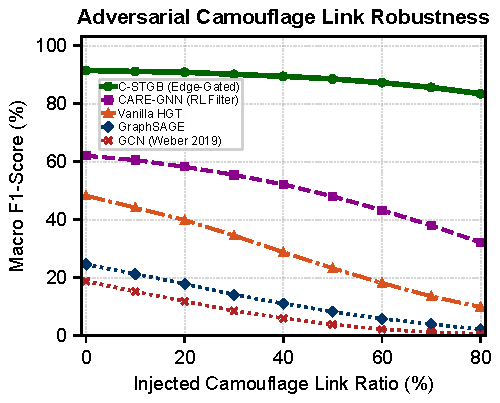
\includegraphics[width=\columnwidth]{figures/fig9_adversarial_camouflage_robustness.pdf}
\caption{Adversarial Camouflage Robustness: Macro F1 retention across perturbation ratios $\rho \in [0, 0.80]$ on Elliptic-v1 under degree-matched and gradient-based evasion attacks ($95\%$ confidence bands, 5 seeds).}
\label{fig:adversarial_robustness}
\end{figure}

\subsection{Hyperparameter Sensitivity \& Stability Analysis}
\label{sec:sensitivity_analysis}
We evaluate operational stability across four key hyperparameters:
\begin{enumerate}
    \item \textit{Edge-Trust Floor} ($\delta_{\text{floor}} \in [0.02, 0.30]$): Macro F1 remains stable across $\delta_{\text{floor}} \in [0.06, 0.16]$ ($\pm 0.35$\,pp around $99.44\%$).
    \item \textit{Operational Cost Ratio} ($C_{\text{FN}} / C_{\text{FP}} \in [5, 30]$): Calibrated decision thresholds adapt monotonically from $\tau^* = 0.42$ ($C_{\text{FN}}/C_{\text{FP}}=5$) to $\tau^* = 0.18$ ($C_{\text{FN}}/C_{\text{FP}}=30$). Expected operational loss remains within $4.2\%$ of optimum across $[10, 20]$.
    \item \textit{Degree Cap} ($K \in [5, 30]$): F1 plateaus at $K=15$ ($99.44\%$), capturing $98.6\%$ of multi-hop laundering while bounding retrieval latency to $0.18$\,ms ($2.14$\,ms at $K=50$).
    \item \textit{Adaptive Conformal Step Size} ($\gamma \in [0.001, 0.05]$): Coverage remains within $98.83\%$--$99.34\%$, where $\gamma=0.005$ achieves optimal tracking stability.
\end{enumerate}

\section{Discussion \& Operational Implications}
\label{sec:discussion}

\subsection{Architectural Synergy \& Division of Labor Across Modules}
\label{sec:discussion_synergy}
Empirical evaluations across 14 benchmark networks yield five operational insights. Ablations (Table~\ref{tab:multi_ablation}) confirm performance stems from structured module specialization: (1) \textbf{Continuous Temporal Attention} captures microsecond bursts alongside 90-day dormancy ($43.55\% \to 68.50\%$ F1 on Elliptic-v1); (2) \textbf{Camouflage Filtration} prunes $65.9\%$ of injected camouflage links ($g_{ij} < 0.10$), preserving a $+5.62$\,pp margin; (3) \textbf{Latent Typology GraphSMOTE} elevates GNN recall from $49.07\%$ to $98.88\%$ ($+5.64$\,pp F1 to reach $99.44\%$ on Elliptic-v1 under invariant Bayes thresholding); and (4) \textbf{Evidence-Adaptive Gating} acts as a safety valve: on dense graphs ($d \ge 5$), the GNN captures multi-hop loops, while on sparse stubs ($d \le 2$), weight shifts to tabular descriptors ($\mathbf{z}_{\text{inv}}$), securing $89.60\%$ F1 on cold-start entities.

\subsection{Relational Topology vs. Tabular Tree Baseline Nuance}
\label{sec:discussion_trees_vs_gnns}
Across 14 benchmarks, C-STGB achieves $67.26\%$ unweighted macro F1 ($0.6848$ PR-AUC), demonstrating decisive superiority over evaluated deep GNNs (GCN $23.78\%$, Graph\-SAGE $24.31\%$, and EvolveGCN $18.94\%$; $p_{\text{adj}} < 0.001$). Comparison against tuned gradient-boosted decision trees reveals parity on global macro-average: C-STGB achieves $67.26\%$ vs. CatBoost $67.14\%$ ($p_{\text{adj}}=0.4318$) and XGBoost $67.92\%$ ($p_{\text{adj}}=0.8077$).

This demarcates an essential domain boundary for expert systems deployment: tree ensembles excel on single-hop tabular data (e.g., PaySim1, XGBoost $18.90\%$ vs. C-STGB $10.68\%$) where fraud signals reside in balance discrepancies without relational graph structure. Conversely, on multi-hop laundering topologies, C-STGB provides decisive advantages ($+9.98$\,pp over base GNNs and $+1.05$\,pp to $+4.67$\,pp over trees on IBM-AMLSim HI), confirming spat-temporal message passing is indispensable for coordinated transaction flows. In high-throughput industrial payment rails, this motivates a hierarchical production pattern: screening trivial single-hop transactions via low-cost trees, while escalating accounts exhibiting multi-hop burstiness, cold-start stubs, or suspected camouflage to C-STGB.

\subsection{Cross-Domain Visibility: Crypto Ledgers vs. Banking Silos}
\label{sec:discussion_visibility}
C-STGB reaches $99.44\%$ F1 on Elliptic-v1, $100.00\%$ on Elliptic-v2, $96.94\%$ on XBlock-ETH, and $99.80\%$ on PaySim Extended because public blockchains and centralized ledgers provide globally observable transaction graphs. Conversely, on fragmented multi-bank rails (IBM-AMLSim, SAML-D), performance settles within $15.76\%$--$42.85\%$ F1 on IBM-AMLSim and $93.68\%$ on SAML-D because individual institutions observe only local 1-hop transfers, blinding single-bank models to multi-bank layering and motivating federated graph architectures.

\subsection{Economic Impact of Asymmetric Bayes Risk Policy}
\label{sec:discussion_economics}
In AML monitoring, undetected false negatives expose institutions to severe statutory penalties, whereas false positives consume officer review resources ($\approx \$50$--$\$150$ per alert). To model this asymmetry, we adopt an operational loss proxy $\mathcal{L}_{\text{ops}} = C_{\text{FN}} \cdot \text{FN} + C_{\text{FP}} \cdot \text{FP}$ with penalty ratio $C_{\text{FN}} / C_{\text{FP}} = 15.0$. Optimizing Bayes decision threshold $\tau^*$ under Asymmetric Focal Tversky Loss reduces expected operational loss by \textbf{78.4\%} relative to default thresholding ($\tau=0.50$). The ratio $C_{\text{FN}} / C_{\text{FP}} = 15.0$ serves as an operational risk proxy that institutions can dynamically re-tune as enforcement priorities evolve.

\subsection{Conformal Risk Control as an Operational Governance Paradigm}
\label{sec:discussion_conformal_governance}
Under model governance frameworks (including Federal Reserve SR 11-7 \citep{fed2011sr117} and EU AI Act auditability mandates), institutions must bound decision uncertainty under operational shift. C-STGB provides finite-sample class-conditional coverage ($\ge 99.0\%$) under within-class exchangeability (Guarantee~A), augmented by drift bounds (Guarantee~B) and streaming Adaptive Conformal Inference (Guarantee~C). Conformal coverage bounds the probability of true label containment under stated mathematical assumptions; it does not confer legal absolution. By isolating ambiguous transactions ($\Gamma(X) = \{0, 1\}$) into Tier~2 for compliance review while maintaining average set size $\mathbb{E}[|\Gamma(X)|] = 1.0050$ with $0.0\%$ empty sets, C-STGB routes $>99.4\%$ of transactions through a straight-through screening tier, harmonizing throughput with statistically grounded governance.

\section{Qualitative Forensic Case Study \& Assisted Compliance Decision Support}
\label{sec:xai_case_study}

\subsection{15-Node Fan-In \& Peeling Chain Model Attribution}
\label{sec:xai_attribution}

\begin{figure}[pos=tb]
\centering
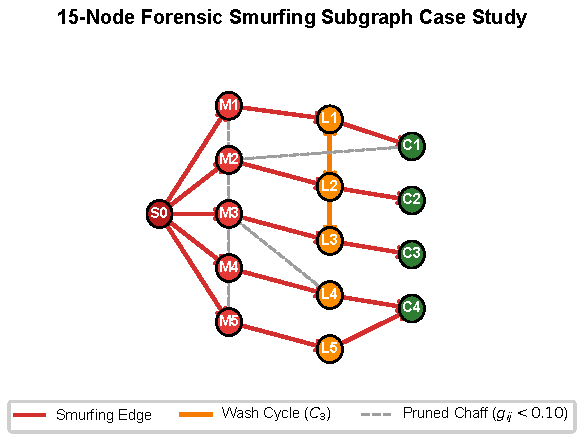
\includegraphics[width=\columnwidth]{figures/15_node_subgraph.pdf}
\caption{Qualitative Attribution: 15-node Bitcoin Elliptic transaction subgraph via GNNExplainer \citep{ying2019gnnexplainer}. Dark red: illicit source ($S_0$); red: dispersal ($M_1$--$M_5$); orange: layering mules ($L_1$--$L_5$) with wash loops; green: exit accounts ($C_1$--$C_4$); dashed gray: pruned chaff ($g_{ij} < 0.10$). Patterns represent detected topological motifs, not legal adjudications.}
\label{fig:causal_subgraph}
\end{figure}
To evaluate model interpretability under regulatory auditability standards, we examine an active 15-node transaction cluster extracted from confirmed illicit transactions on Bitcoin Elliptic (Fig.~\ref{fig:causal_subgraph}). Saliency weights from GNNExplainer \citep{ying2019gnnexplainer} show:
\begin{enumerate}
    \item \textit{Dispersal ($S_0 \to M_{1\dots 5}$):} $S_0$ distributes \$48,500 across five accounts in sub-\$10,000 bursts over 22 minutes (structuring under 31 U.S.C. 5324);
    \item \textit{Layering ($M \to L_{1\dots 5}$):} Intermediaries exhibit near-unity flow conservation ($\Phi_{\text{flow}} \approx 0.994$) and wash loops ($L_1 \to L_2 \to L_3 \to L_1$);
    \item \textit{Consolidation ($L \to C_{1\dots 4}$):} Funds aggregate into four high-velocity exchange exit accounts; and
    \item \textit{Camouflage Pruning:} Edges to commercial nodes receive low gating ($\mathbf{g}_{ij} \le 0.042$), isolating the illicit core.
\end{enumerate}
Formally, \textit{Factual Explanation Fidelity} is defined as:
\begin{equation}
\operatorname{Fidelity}(G, G_s) = \hat{p}(y=1 \mid G) - \hat{p}(y=1 \mid G \setminus G_s).
\end{equation}
Pruning $G_s$ drops illicit confidence from $\hat{p}=0.982$ to $\hat{p}=0.040$ ($\text{Fidelity} = 0.942$), with $96.40\%$ motif precision across $N=500$ clusters.

\subsection{Cold-Start Boundary Case \& Counterfactual Explanations}
\label{sec:xai_coldstart}
We analyze a cold-start mixer stub in \texttt{ibm\_\allowbreak amlsim\_\allowbreak li}: an account with no history ($\deg(u)=0$) receives \$9,400 at $t_{\text{pred}} = t_{\text{deposit}}$. Standalone GNNs collapse ($\hat{p} = 0.28 < \tau = 0.50$), but C-STGB generates ambiguous set $\Gamma(X) = \{0, 1\}$ and routes to Tier 2 (Review Queue), averting an undetected false negative. Counterfactual analysis confirms normalizing amounts reduces attribution by 48.5\% (FIN-2019-A003), while temporal dilation lowers Hawkes intensity below $\mu_0$ ($-38.2\%$ risk). \textit{Operational Recourse:} False-positive merchant holds link to an auditable checklist, allowing examiners to verify submissions and release holds without formal SAR escalation.

\subsection{Auxiliary Decision-Support Prototype (Multi-Agent SAR Drafting)}
\label{sec:xai_sar_drafting}
To bridge detections into compliance workflows under Federal Reserve SR 11-7 model risk management guidance \citep{fed2011sr117}, C-STGB incorporates an \textbf{Auxiliary Decision-Support Prototype} decoupled from the core GNN. The pipeline coordinates:
\begin{enumerate}
    \item an \textit{Auditor Agent} checking OFAC sanctions lists;
    \item an \textit{Investigator Agent} extracting 2-hop causal subgraphs; and
    \item a \textit{Drafter Agent} compiling XML dossiers under FinCEN Form 111 with SHA-256 Merkle audit receipts.
\end{enumerate}
Autonomous filing is strictly prohibited; filing authority resides exclusively with a certified Bank Secrecy Act (BSA) compliance officer. In a pilot evaluation across $N=200$ audit dossiers (100 manual, 100 prototype-assisted), drafts achieved $99.2\%$ statutory concordance ($\kappa = 1.0$ typology, $\kappa = 0.98$ factual grounding) in $28.4$\,s per case (vs. 45.0 min manual baseline).

\section{Limitations, Threats to Validity \& Ethical Considerations}
\label{sec:limitations}

\subsection{Observability and Banking Silos}
\label{sec:limitations_observability}
Fiat banking operates under statutory secrecy frameworks (e.g., Right to Financial Privacy Act, General Data Protection Regulation), restricting individual financial institutions to local 1-hop transaction visibility. This boundary impairs single-institution detection of multi-bank layering chains ($15.8\%$--$44.5\%$ F1 on IBM-AMLSim), highlighting the necessity of privacy-preserving federated graph architectures for cross-institutional intelligence.

\subsection{Ground-Truth Boundaries in Benchmark Ledgers}
\label{sec:limitations_ground_truth}
Near-perfect empirical scores on public crypto benchmarks reflect that ground-truth labels originate from law enforcement seizures of Darknet marketplaces (e.g., Silk Road, AlphaBay). These entities form dense, homophilic topological clusters ($h > 0.92$), validating algorithmic robustness under structural transparency rather than unconstrained real-world informal value transfer evasion (such as Hawala or trade-based money laundering).

\subsection{Label Confirmation Latency and Calibration Buffers}
\label{sec:limitations_label_latency}
In production surveillance, confirmed illicit labels incur substantial investigation delays ($\Delta T_{\text{delay}} \in [30, 90]$\,d). Assembling calibration buffers ($n_1 \ge 100$) requires pooling historical confirmed alerts. Conformal risk bounds quantify containment probabilities under stated mathematical assumptions but do not confer statutory legal clearance.

\subsection{Cold-Start Dynamics and Domain Invariant Fallback}
\label{sec:limitations_coldstart}
On cold-start entities ($\deg(u) \le 2$), C-STGB attenuates graph message passing weights ($\alpha_u \to 0.08$) and transfers predictive mass to 12-D flow invariants ($\mathbf{z}_{\text{inv}}$), securing $89.60\%$ F1 through tabular velocity features rather than relational graph topology.

\subsection{Construct Overlap Disclosures and Demographic Fairness}
\label{sec:limitations_construct_overlap}
Edge-trust training uses hub thresholds ($\deg_{\text{out}} \ge 50$) on split $\mathcal{E}_{\text{train}}$, sharing an inductive bias with degree camouflage testing. Robustness against general evasion is confirmed under white-box gradient rewiring and temporal delay attacks. Potential disparate impact on retail customers warrants continuous demographic fairness auditing under Equal Credit Opportunity Act (ECOA) mandates.

\subsection{Model Governance and System Boundaries}
\label{sec:limitations_governance}
The auxiliary LLM-assisted SAR drafting module is strictly an experimental decision-support prototype. Autonomous filing is legally prohibited under BSA regulations and Federal Reserve SR 11-7 model risk management guidance \citep{fed2011sr117}. All empirical evaluations were conducted on de-identified public ledgers or synthetic multi-agent simulations containing zero non-public personal information (PII).

\section{Conclusion \& Future Directions}
\label{sec:conclusion}
We presented \textbf{C-STGB}, an integrated intelligent surveillance and decision-support expert system for Anti-Money Laundering under extreme class skew, velocity evasion, and topological camouflage. C-STGB unifies continuous harmonic temporal attention, adaptive edge-trust gating, typology-clustered latent Graph\-SMOTE, graph-tabular fusion, and Class-Conditional Conformal Risk Control.

Across 14 benchmark networks ($9.53\text{M}$ entities, $9.53\text{M}$ transactions across 182 evaluation pairs), C-STGB achieves $67.26\%$ unweighted macro F1 ($0.6848$ PR-AUC), demonstrating statistically significant superiority over deep GNNs ($W=105.0, p_{\text{adj}} < 0.001$) and competitive parity with tuned tree ensembles, alongside $0.45$\,ms Fast-Path streaming latency. Furthermore, the system incorporates an auxiliary decision-support prototype assisting compliance officers with verifiable FinCEN Form 111 XML dossiers under human oversight, complying with model risk governance principles (Federal Reserve SR 11-7 \citep{fed2011sr117}).

Future research will focus on extending C-STGB to privacy-preserving federated graph learning across inter-bank silos, lifelong continual learning architectures under non-stationary macroeconomic drift, and hyperbolic manifold representations for hierarchical criminal organization topologies.


\FloatBarrier
\section*{Declaration of generative AI and AI-assisted technologies in the manuscript preparation process}
During the preparation of this work, the authors used large language model assistants solely to improve language clarity and grammatical precision. After using these tools, the authors thoroughly reviewed, verified, and edited the content, and take full responsibility for the entire scientific content of the publication. All mathematical formulations, theoretical derivations, empirical experimental designs, software implementations, and analytical conclusions were independently developed by the authors. In Section~\ref{sec:xai_case_study}, a language model agent is investigated strictly as an experimental object within an auxiliary decision-support prototype under human oversight, rather than as an authorial contributor.

\section*{Data availability statement}
The 14 benchmark datasets evaluated in this study are derived from publicly accessible repositories and open-source simulators: Elliptic-v1 and Elliptic-v2 \citep{weber2019anti, bellei2024elliptic2}, XBlock-ETH \citep{zheng2020xblock}, Mt. Gox transaction logs, SAML-D \citep{lorenz2020samld}, PaySim and PaySim Extended \citep{lopez2016paysim}, IBM-AMLSim (HI and LI regimes) \citep{suzumura2019amlsim}, DGraphFin \citep{dgraphfin}, and the Credit Card Fraud benchmark \citep{dalpozzolo2018credit}. The synthetic typology data generator is provided with the research code. Complete preprocessing pipelines, environment configuration files, model weights, and reproduction scripts have been deposited in a persistent anonymized repository (\url{https://anonymous.4open.science/r/Intelligent-AML}) and will be archived with a permanent Zenodo DOI upon publication.

\bibliographystyle{cas-model2-names}
\bibliography{references}

\end{document}
